\documentclass[12pt,a4paper,oneside]{report}

\usepackage[a4paper,top=2cm,bottom=2cm,left=3cm,right=2cm,headheight=14pt,headsep=1cm,footskip=1cm]{geometry}
\usepackage{fontspec}
\IfFontExistsTF{Times New Roman}{\setmainfont{Times New Roman}}{\setmainfont{Liberation Serif}}
\usepackage{setspace}
\usepackage{ragged2e}
\usepackage{titlesec}
\usepackage{fancyhdr}
\usepackage[xetex]{graphicx}
\usepackage{tabularx}
\usepackage{longtable}
\usepackage{url}
\usepackage{array}
\usepackage{booktabs}
\usepackage{caption}
\usepackage{float}
\usepackage{newfloat}

\DeclareFloatingEnvironment[within=chapter,fileext=lod,listname={DANH MỤC SƠ ĐỒ},name={Sơ đồ}]{diagram}
\newcolumntype{Y}{>{\RaggedRight\arraybackslash}X}
\newcolumntype{L}[1]{>{\RaggedRight\arraybackslash}p{#1}}

\setcounter{tocdepth}{3}
\setlength{\parskip}{3pt}
\setlength{\parindent}{1.27cm}
\setstretch{1.15}
\justifying

\titleformat{\chapter}[hang]
  {\normalfont\bfseries\fontsize{14}{17}\selectfont}
  {\MakeUppercase{\chaptername~\thechapter:}}
  {0.6em}
  {\MakeUppercase}
\titleformat{\section}
  {\normalfont\bfseries\fontsize{13}{16}\selectfont}
  {\thesection}{0.6em}{}
\titleformat{\subsection}
  {\normalfont\bfseries\fontsize{13}{16}\selectfont}
  {\thesubsection}{0.6em}{}
\titlespacing*{\chapter}{0pt}{0pt}{12pt}

\pagestyle{fancy}
\fancyhf{}
\fancyhead[L]{\small Đồ án tốt nghiệp Đại học}
\fancyhead[R]{\small\nouppercase{\leftmark}}
\fancyfoot[L]{\footnotesize Nguyễn Lưu Tấn Sang; Vũ Ngọc Sơn; Đỗ Xuân Trí -- D22CQCNPM01-N}
\fancyfoot[R]{\small\thepage}
\renewcommand{\headrulewidth}{0.4pt}
\renewcommand{\footrulewidth}{0pt}
\renewcommand{\chaptermark}[1]{\markboth{\ifnum\value{chapter}>0 \chaptername~\thechapter: \MakeUppercase{#1}\else #1\fi}{}}
\fancypagestyle{plain}{%
  \fancyhf{}
  \fancyhead[L]{\small Đồ án tốt nghiệp Đại học}
  \fancyhead[R]{\small\nouppercase{\leftmark}}
  \fancyfoot[L]{\footnotesize Nguyễn Lưu Tấn Sang; Vũ Ngọc Sơn; Đỗ Xuân Trí -- D22CQCNPM01-N}
  \fancyfoot[R]{\small\thepage}
  \renewcommand{\headrulewidth}{0.4pt}
}

\captionsetup{font=normalsize,labelfont=bf,justification=centering}

\newcommand{\projecttitle}{Hệ thống quản lý ứng phó khẩn cấp và cứu trợ thiên tai}
\newcommand{\advisorname}{ThS. Trương Thị Mỹ Ngọc}
\newcommand{\reportyear}{2026}
\newcommand{\frontchapter}[1]{%
  \chapter*{#1}%
  \addcontentsline{toc}{chapter}{#1}%
  \markboth{#1}{}%
}
\newcommand{\makecover}{%
  \begin{titlepage}
    \thispagestyle{empty}
    \begin{center}
      {\bfseries BỘ KHOA HỌC VÀ CÔNG NGHỆ\par}
      \vspace{0.15cm}
      {\bfseries HỌC VIỆN CÔNG NGHỆ BƯU CHÍNH VIỄN THÔNG\par}
      \vspace{0.12cm}
      {\small\makebox[9cm]{\leaders\hbox{--}\hfill}\par}
      \vspace{0.25cm}
      
\includegraphics[height=3.2cm]{images/ptit-logo.jpg}\par
      \vspace{0.35cm}
      {\bfseries\fontsize{36}{42}\selectfont ĐỒ ÁN\par}
      {\bfseries\fontsize{36}{42}\selectfont TỐT NGHIỆP ĐẠI HỌC\par}
      \vspace{0.45cm}
      \begin{minipage}{\textwidth}
        \raggedright\bfseries\itshape Đề tài:\par
      \end{minipage}\par
      \vspace{0.2cm}
      {\bfseries\itshape\fontsize{16}{20}\selectfont\MakeUppercase{\projecttitle}\par}
      \vspace{1.6cm}
      \begin{minipage}{\textwidth}
        \bfseries\fontsize{13}{16}\selectfont
        \setlength{\tabcolsep}{3pt}
        \renewcommand{\arraystretch}{1.15}
        \begin{tabularx}{\textwidth}{@{}L{4.8cm}Y L{1.6cm}L{3.0cm}@{}}
          Giảng viên hướng dẫn: & \multicolumn{3}{l}{\MakeUppercase{\advisorname}} \\
          Sinh viên thực hiện: & \MakeUppercase{Nguyễn Lưu Tấn Sang} & MSSV: & N22DCCN068 \\
          & \MakeUppercase{Vũ Ngọc Sơn} & MSSV: & N22DCCN071 \\
          & \MakeUppercase{Đỗ Xuân Trí} & MSSV: & N22DCCN088 \\
          Lớp: & \multicolumn{3}{l}{D22CQCNPM01-N} \\
          Ngành: & \multicolumn{3}{l}{Công nghệ thông tin} \\
        \end{tabularx}
      \end{minipage}
      \vfill
      {\bfseries TP. HỒ CHÍ MINH, NĂM \reportyear\par}
    \end{center}
  \end{titlepage}%
}
\newcommand{\mobilescreenshot}[3]{%
  \begin{figure}[H]
    \centering
    \includegraphics[width=0.39\textwidth,height=0.67\textheight,keepaspectratio]{#1}
    \caption{#2}\label{#3}
  \end{figure}%
}

\begin{document}
\renewcommand{\chaptername}{CHƯƠNG}
\renewcommand{\figurename}{Hình}
\renewcommand{\tablename}{Bảng}
\renewcommand{\contentsname}{MỤC LỤC}
\renewcommand{\listtablename}{DANH MỤC CÁC BẢNG}
\renewcommand{\listfigurename}{DANH MỤC HÌNH VẼ}
\renewcommand{\bibname}{TÀI LIỆU THAM KHẢO}

% Trang lót trắng là yêu cầu in ấn; bìa vật lý cần hoàn thiện riêng khi đóng quyển.
\makecover
\null\thispagestyle{empty}\newpage
\makecover

% Trang giao nhiệm vụ chờ bản được phê duyệt; số La Mã bắt đầu từ lời cảm ơn.
\pagenumbering{gobble}
\chapter*{PHÊ DUYỆT, GIAO NHIỆM VỤ ĐỀ TÀI}
\markboth{PHÊ DUYỆT, GIAO NHIỆM VỤ ĐỀ TÀI}{}
\noindent[ Bổ sung bản giao nhiệm vụ đã được phê duyệt và ký xác nhận vào trang này. ]\par
\vfill
\noindent\begin{tabularx}{\textwidth}{Y Y}
  \centering GIẢNG VIÊN HƯỚNG DẪN & \centering ĐẠI DIỆN NHÓM SINH VIÊN\tabularnewline
  \centering (Ký và ghi rõ họ tên) & \centering (Ký và ghi rõ họ tên)
\end{tabularx}

\clearpage
\pagenumbering{roman}
\frontchapter{LỜI CẢM ƠN}
Trong quá trình thực hiện đề tài quản lý ứng phó khẩn cấp và cứu trợ thiên tai, nhóm có dịp vận dụng kiến thức đã học vào một bài toán đòi hỏi nhiều bên phối hợp. Từ việc tiếp nhận thông tin đến xác minh, giao nhiệm vụ và theo dõi hàng cứu trợ, mỗi bước đều cần được ghi nhận rõ ràng để người tham gia hiểu việc gì đã được xử lý và việc gì còn tiếp tục. Quá trình tìm hiểu cũng giúp nhóm nhận ra rằng một giải pháp công nghệ chỉ có ý nghĩa khi thông tin được tổ chức cẩn thận và quyền riêng tư của người cần trợ giúp được tôn trọng.

Nhóm xin cảm ơn Ban Giám đốc Học viện Công nghệ Bưu chính Viễn thông, các thầy cô và cán bộ Học viện đã tạo điều kiện để sinh viên học tập, nghiên cứu và thực hiện đồ án. Những kiến thức về công nghệ thông tin, phân tích và thiết kế hệ thống, cơ sở dữ liệu và phát triển phần mềm đã giúp nhóm có nền tảng để tiếp cận đề tài.

Nhóm đặc biệt cảm ơn cô ThS. Trương Thị Mỹ Ngọc, giảng viên hướng dẫn, vì đã dành thời gian định hướng và góp ý cho nhóm trong quá trình thực hiện. Những nhận xét của cô giúp nhóm xem xét bài toán có hệ thống hơn, chú ý mối liên hệ giữa yêu cầu, quy trình xử lý, dữ liệu và kết quả cần trình bày. Nhóm cũng trân trọng sự kiên nhẫn và những lời động viên của cô trong những lúc nhóm cần rà soát, điều chỉnh lại nội dung.

Nhóm xin cảm ơn các thành viên đã cùng trao đổi, chia sẻ công việc và hỗ trợ nhau hoàn thành những phần còn vướng; cảm ơn gia đình và người thân đã quan tâm, động viên trong suốt thời gian thực hiện đồ án. Nhóm cũng ghi nhận các tài liệu chuyên môn đã giúp làm rõ thêm những vấn đề liên quan đến đề tài.

Với thời gian và kinh nghiệm còn hạn chế, đồ án vẫn có thể còn thiếu sót. Nhóm mong nhận được góp ý của cô hướng dẫn và quý thầy cô để tiếp tục hoàn thiện nội dung và sản phẩm. Nhóm xin chân thành cảm ơn.
\vfill
\begin{flushright}
  TP. Hồ Chí Minh, ngày [..] tháng [..] năm [....]\\[0.8cm]
  \textbf{ĐẠI DIỆN NHÓM SINH VIÊN}\\[0.8cm]
  (Ký và ghi rõ họ tên)
\end{flushright}

\frontchapter{LỜI CAM ĐOAN}
Chúng em xin cam đoan đồ án này do các thành viên trong nhóm thực hiện dưới sự hướng dẫn của cô ThS. Trương Thị Mỹ Ngọc. Nội dung, số liệu và kết quả trình bày trong báo cáo được ghi nhận trung thực theo quá trình tìm hiểu, thiết kế và xây dựng sản phẩm của nhóm.

Những nội dung tham khảo từ tài liệu, công trình hoặc nguồn khác đều được trích dẫn trong báo cáo. Nhóm xin chịu trách nhiệm về lời cam đoan này và về tính chính xác của các nội dung do mình trình bày.
\vfill
\begin{flushright}
  TP. Hồ Chí Minh, ngày [..] tháng [..] năm [....]\\[1cm]
  \textbf{ĐẠI DIỆN NHÓM SINH VIÊN}\\
  (Ký và ghi rõ họ tên)
\end{flushright}

\clearpage
\addcontentsline{toc}{chapter}{MỤC LỤC}
\tableofcontents

\frontchapter{DANH MỤC CÁC KÝ HIỆU VÀ CHỮ VIẾT TẮT}
\small
\begin{tabularx}{\textwidth}{@{}l X X@{}}
  \toprule
  \textbf{Ký hiệu} & \textbf{Tên đầy đủ} & \textbf{Nghĩa tiếng Việt} \\
  \midrule
  AI & Artificial Intelligence & Trí tuệ nhân tạo \\
  API & Application Programming Interface & Giao diện lập trình ứng dụng \\
  ERD & Entity-Relationship Diagram & Sơ đồ thực thể -- liên kết \\
  FE & Frontend & Phần giao diện phía người dùng \\
  FR & Functional Requirement & Yêu cầu chức năng \\
  GPS & Global Positioning System & Hệ thống định vị toàn cầu \\
  NFR & Non-functional Requirement & Yêu cầu phi chức năng \\
  PostGIS & PostgreSQL Geographic Information System & Phần mở rộng dữ liệu địa lý cho \mbox{PostgreSQL} \\
  RBAC & Role-Based Access Control & Kiểm soát truy cập dựa trên vai trò \\
  SDD & Software Design Description & Tài liệu mô tả thiết kế phần mềm \\
  SOS & Emergency assistance request & Yêu cầu trợ giúp khẩn cấp \\
  SRS & Software Requirements Specification & Đặc tả yêu cầu phần mềm \\
  TC & Test Case & Ca kiểm thử \\
  UC & Use Case & Ca sử dụng \\
  UI/UX & User Interface / User Experience & Giao diện và trải nghiệm người dùng \\
  UR & User Requirement & Yêu cầu người dùng \\
  \bottomrule
\end{tabularx}
\normalsize

\clearpage
\addcontentsline{toc}{chapter}{\listtablename}
\listoftables
\clearpage
\addcontentsline{toc}{chapter}{DANH MỤC SƠ ĐỒ}
\listofdiagrams
\clearpage
\addcontentsline{toc}{chapter}{\listfigurename}
\listoffigures

\clearpage
\pagenumbering{arabic}
\frontchapter{MỞ ĐẦU}
Trong tình huống thiên tai, thông tin về người cần trợ giúp, vị trí hiện trường và nguồn lực cứu hộ thường thay đổi nhanh. Khi các thông tin này được ghi nhận ở nhiều nơi, việc xác minh yêu cầu, phân công đội ứng cứu và theo dõi hàng cứu trợ trở nên khó khăn. Từ yêu cầu đó, nhóm thực hiện đề tài xây dựng một hệ thống hỗ trợ phối hợp giữa người dân, đội ứng cứu, điều phối viên và đơn vị quản lý.

Các tài liệu nền của đề tài tập trung vào yêu cầu, kiến trúc và những quy trình chính cần hỗ trợ. Báo cáo kế thừa các nội dung đó để phân tích giải pháp và cách tổ chức hệ thống; việc đối chiếu sâu với các hệ thống cứu trợ đang vận hành chưa thuộc phạm vi thực hiện.

Mục tiêu của đề tài là phân tích các quy trình chính, xác định yêu cầu của từng nhóm người dùng, thiết kế kiến trúc và dữ liệu, đồng thời xây dựng các chức năng backend phục vụ tiếp nhận yêu cầu, điều phối nhiệm vụ và quản lý cứu trợ. Báo cáo cũng nêu rõ những phần đã triển khai và những nội dung còn cần kiểm chứng trước khi đánh giá toàn bộ sản phẩm.

Nhóm thực hiện đề tài bằng cách phân tích yêu cầu được giao và tài liệu kỹ thuật, mô hình hóa tác nhân và ca sử dụng, sau đó đối chiếu các yêu cầu với thiết kế, mã nguồn và kết quả kiểm thử đã ghi nhận. Nhóm chưa phỏng vấn trực tiếp người dân hoặc lực lượng ứng cứu; vì vậy, các nội dung về quy trình thực tế được trình bày như yêu cầu cần xác nhận, không phải kết quả khảo sát thực địa.

\textbf{Kết cấu:} Chương 1 giới thiệu đề tài; Chương 2 khảo sát bối cảnh và tác nhân; Chương 3 phân tích, thiết kế và xây dựng backend; Chương 4 trình bày tổ chức dữ liệu; Chương 5 và Chương 6 lần lượt mô tả thiết kế giao diện Web và ứng dụng di động; Chương 7 tổng kết kết quả và kiến nghị.

\frontchapter{BẢNG PHÂN CÔNG NHIỆM VỤ NHÓM THỰC HIỆN}
Nhóm phân chia công việc theo các mảng chuyên môn, đồng thời phối hợp trong những nội dung cần thống nhất chung. Nguyễn Lưu Tấn Sang tập trung rà soát thiết kế và xây dựng Backend; Vũ Ngọc Sơn và Đỗ Xuân Trí cùng phụ trách UI/UX, Web/Mobile và Frontend. Cả ba thành viên cùng trao đổi về yêu cầu, ca sử dụng, mô hình dữ liệu và nội dung báo cáo.
\begin{table}[htbp]
  \centering
  \caption{Phân công nhiệm vụ của nhóm thực hiện}\label{tab:task-assignment}
  \small
  \begin{tabularx}{\textwidth}{@{}L{3.6cm}L{3.7cm}Y@{}}
    \toprule
    \textbf{Mã SV -- Họ tên} & \textbf{Luồng công việc} & \textbf{Phạm vi nhiệm vụ} \\
    \midrule
    N22DCCN068 -- Nguyễn Lưu Tấn Sang & Thiết kế hệ thống và Backend & Rà soát thiết kế, mô hình dữ liệu và xây dựng các dịch vụ Backend. \\
    N22DCCN071 -- Vũ Ngọc Sơn & UI/UX, Web/Mobile và Frontend & Cùng thiết kế trải nghiệm và xây dựng các giao diện Web/Mobile. \\
    N22DCCN088 -- Đỗ Xuân Trí & UI/UX, Web/Mobile và Frontend & Cùng thiết kế trải nghiệm và xây dựng các giao diện Web/Mobile. \\
    Cả ba thành viên & Rà soát chung & Thống nhất tác nhân, use case, ERD, phạm vi và truy vết yêu cầu. \\
    \bottomrule
  \end{tabularx}
  \par\small\textit{Nguồn:} Nhóm thực hiện tổng hợp theo phân công công việc trong kế hoạch kỹ thuật.
\end{table}



\chapter{GIỚI THIỆU ĐỀ TÀI}\label{ch:introduction}
\section{Sự cần thiết của đề tài}
Trong các tình huống như lũ lụt, bão và sạt lở, người dân, tình nguyện viên, đội cứu hộ, điều phối viên và đơn vị quản lý cần trao đổi thông tin về hiện trường, nhiệm vụ và nguồn lực. Khi thông tin đến từ nhiều kênh, các bên có thể khó xác định yêu cầu nào đã được tiếp nhận, ai đang xác minh, đội nào đã nhận nhiệm vụ và phần hỗ trợ nào còn thiếu. Vì vậy, bài toán không chỉ là ghi nhận thông tin ban đầu mà còn là theo dõi thông tin đó xuyên suốt quá trình xử lý.

Hệ thống được thiết kế để tập trung thông tin và hỗ trợ phối hợp giữa các bên. Khi một người báo giúp hộ khác, thông tin của người báo cần được tách khỏi thông tin của hộ cần trợ giúp; vị trí và dữ liệu liên hệ chỉ nên hiển thị cho người có nhiệm vụ phù hợp. Việc xác minh, lựa chọn mức ưu tiên và giao đội vẫn do người có thẩm quyền quyết định.

\section{Mục tiêu của đề tài}
Mục tiêu tổng quát là xây dựng một hệ thống Web/Mobile quản lý ứng phó khẩn cấp và cứu trợ thiên tai, hỗ trợ phối hợp từ lúc ghi nhận thông tin đến khi theo dõi nhiệm vụ và nguồn lực. Các mục tiêu cụ thể gồm:
\begin{enumerate}
  \item Tiếp nhận SOS/yêu cầu trợ giúp có loại tình huống, vị trí GPS hoặc ghim thủ công, thông tin liên hệ và bằng chứng tùy chọn.
  \item Hỗ trợ điều phối viên xem hàng đợi, ghi nhận xác minh, xử lý báo trùng có lý do, quyết định mức ưu tiên và giao nhiệm vụ.
  \item Hỗ trợ đội/tình nguyện viên xem nhiệm vụ thuộc phạm vi của mình, cập nhật tiến độ và gửi bằng chứng kết quả.
  \item Theo dõi chiến dịch, điểm tiếp nhận, kho, vật tư, phương tiện và phân phối cứu trợ ở mức cần cho các luồng cốt lõi.
  \item Cho phép người dân khai báo hàng hóa đã bàn giao; nhân viên tiếp nhận kiểm đếm và một người khác thẩm định độc lập trước khi ghi nhận hàng vào tồn kho.
  \item Cung cấp bản đồ và báo cáo có phạm vi, bộ lọc và thời điểm tạo dữ liệu rõ ràng; bảo vệ vị trí và thông tin liên hệ nhạy cảm.
\end{enumerate}
AI, thông báo đẩy và các chức năng ngoại tuyến sâu là phần mở rộng có điều kiện. Nếu có gợi ý AI, quyết định ưu tiên, xác minh và điều phối vẫn do người có thẩm quyền thực hiện; phần lõi phải dùng được khi AI tắt.

\section{Mục tiêu sản phẩm và phạm vi báo cáo}
Phạm vi đề tài gồm sản phẩm Web/Mobile và các tài liệu SRS, SDD, ca kiểm thử, hướng dẫn người dùng, hướng dẫn cài đặt. Backend đã có các chức năng quản lý tài khoản và quyền, tiếp nhận và điều phối yêu cầu, quản lý đội ứng cứu, chiến dịch, hàng cứu trợ, tồn kho và phân phối. Giao diện Web đã tích hợp các luồng chính với API và được trình bày cùng ảnh chụp từ hệ thống demo ở Chương~\ref{ch:web}. Phần Mobile tiếp tục mô tả luồng và nguyên tắc giao diện; ảnh thiết bị thực tế còn cần bổ sung ở Chương~\ref{ch:mobile}.

Một số nội dung vận hành vẫn cần được hoàn thiện hoặc kiểm chứng, gồm quyền truy cập tệp riêng tư, sao lưu và khôi phục, tác vụ định kỳ, hiệu năng trên dữ liệu đại diện, cùng các tài liệu bàn giao độc lập.

\begin{table}[htbp]
  \centering
  \caption{Phạm vi chức năng của sản phẩm}\label{tab:scope-priority}
  \small
  \begin{tabularx}{\textwidth}{@{}L{3.0cm}Y L{4.0cm}@{}}
    \toprule
    \textbf{Nhóm chức năng} & \textbf{Nội dung} & \textbf{Giới hạn phạm vi} \\
    \midrule
    Tiếp nhận yêu cầu & Gửi SOS cho bản thân hoặc báo giúp hộ gia đình; ghi nhận loại tình huống, vị trí, thông tin liên hệ và bằng chứng; theo dõi, bổ sung thông tin. & Báo giúp hộ gia đình phân biệt người báo với người cần trợ giúp. \\
    Điều phối ứng cứu & Xác minh yêu cầu, xem xét báo trùng, đặt ưu tiên, giao đội và theo dõi tiến độ, kết quả nhiệm vụ. & Xác minh, ưu tiên và điều phối do người có thẩm quyền quyết định. \\
    Quản lý cứu trợ & Quản lý chiến dịch, điểm tiếp nhận, hàng quyên góp, kiểm đếm, duyệt độc lập, tồn kho và phân phối. & Trong phạm vi là hàng hóa; không gồm thu tiền hoặc thanh toán. \\
    Theo dõi vận hành & Bản đồ, hàng đợi, báo cáo và lịch sử thao tác theo phạm vi quyền. & Dữ liệu vị trí và thông tin liên hệ nhạy cảm cần được giới hạn truy cập. \\
    Chức năng mở rộng & Gợi ý AI, thông báo đẩy và thao tác ngoại tuyến nâng cao. & Là hướng mở rộng; không thay thế quyết định của con người và chưa thuộc phạm vi chức năng đã xây dựng. \\
    \bottomrule
  \end{tabularx}
  \par\small\textit{Nguồn:} Nhóm thực hiện tổng hợp từ yêu cầu đề tài và phạm vi thiết kế.
\end{table}

\section{Đối tượng và phương pháp nghiên cứu}
Đối tượng nghiên cứu là quy trình thông tin và phần mềm phục vụ tiếp nhận yêu cầu trợ giúp, điều phối đội ứng cứu, quản lý chiến dịch và theo dõi cứu trợ hiện vật. Nhóm người dùng được phân tích tại Mục~\ref{sec:actors}. Phương pháp gồm phân tích tài liệu được giao, tách yêu cầu gốc khỏi lựa chọn thiết kế, mô hình hóa tác nhân/use case, xác lập mã truy vết và đối chiếu yêu cầu với tài liệu, mã nguồn và hồ sơ kiểm chứng.

Nhóm chưa phỏng vấn trực tiếp người dân hoặc lực lượng ứng cứu. Các ngưỡng quá hạn, mức ưu tiên P1--P4, số lần liên hệ và thời hạn lưu dữ liệu vì vậy được trình bày như phương án thiết kế; đơn vị nghiệp vụ cần xác nhận trước khi áp dụng.

\chapter{KHẢO SÁT HỆ THỐNG}\label{ch:survey}
\section{Bối cảnh và vấn đề cần khảo sát}
Lũ lụt, bão, sạt lở và các sự cố khác có thể làm phát sinh nhiều yêu cầu trợ giúp trong thời gian ngắn. Từ yêu cầu đề tài, nhóm tập trung vào những vấn đề cần được làm rõ khi ghi nhận và xử lý thông tin: vị trí hoặc thời điểm có thể chưa đầy đủ, các báo cáo gần nhau có thể thuộc cùng một hộ, người báo cần biết yêu cầu đang ở bước nào, và số hàng đã phân phối cần đối chiếu được với số hàng tiếp nhận. Đây là những vấn đề làm cơ sở cho phần phân tích và thiết kế ở các chương sau.\cite{ocha-hpc,wfp-warehouse}

\section{Mục tiêu khảo sát}
Khảo sát cần làm rõ: (1) thông tin tối thiểu để tiếp nhận một báo cáo; (2) cách xác minh nguồn tin và xử lý trường hợp không liên lạc được; (3) ai có quyền đặt ưu tiên, giao nhiệm vụ và xác nhận kết quả; (4) cách các đội ngoài ứng dụng báo tiến độ; (5) cách kiểm đếm, duyệt độc lập và bàn giao hàng hóa; (6) dữ liệu nào được hiển thị trên bản đồ/báo cáo; và (7) điều kiện kết nối yếu, bảo mật và lưu trữ dữ liệu.

\section{Các tác nhân của hệ thống}\label{sec:actors}
\begin{table}[htbp]
  \centering
  \caption{Tác nhân và nhu cầu thông tin chính}\label{tab:actors}
  \small
  \begin{tabularx}{\textwidth}{@{}L{3.1cm}Y Y@{}}
    \toprule
    \textbf{Tác nhân} & \textbf{Nhu cầu chính} & \textbf{Phạm vi dữ liệu/hoạt động dự kiến} \\
    \midrule
    Người dân & Gửi yêu cầu trợ giúp, biết máy chủ đã nhận hay chưa, theo dõi trạng thái và bổ sung thông tin khi được phép. & Chỉ xem yêu cầu của mình hoặc dùng bí mật theo dõi riêng cho yêu cầu khách. \\
    Tình nguyện viên/đội cứu hộ & Xem nhiệm vụ được giao, chấp nhận/từ chối, cập nhật tiến độ và báo kết quả. & Chỉ xem nhiệm vụ thuộc đội và phạm vi được cấp; quyền sửa phụ thuộc vai trò đội trưởng. \\
    Điều phối viên & Xác minh báo cáo, rà soát trùng, lựa chọn ưu tiên, giao đội và theo dõi hoạt động trên bản đồ. & Dữ liệu đúng tổ chức/vùng và quyền tác vụ; quyết định được lưu dấu vết. \\
    Quản lý vận hành/chiến dịch & Quản lý chiến dịch, điểm cứu trợ, kho, phương tiện và tổng hợp hoạt động. & Thao tác vật tư và báo cáo trong phạm vi được cấp; không mặc nhiên có quyền xem mọi vị trí cá nhân. \\
    Quản trị viên hệ thống & Quản lý tài khoản, tổ chức, quyền truy cập và hoạt động hệ thống. & Quyền quản trị được tách khỏi quyền nghiệp vụ; thao tác cấp quyền có kiểm toán. \\
    Đơn vị/cơ quan phối hợp bên ngoài & Có thể là nguồn hoặc nơi tiếp nhận thông tin khi phối hợp ứng cứu. & Việc cấp tài khoản cho các đơn vị bên ngoài chưa nằm trong phạm vi xác định; hệ thống chưa xem họ là người dùng nội bộ. \\
    \bottomrule
  \end{tabularx}
  \par\small\textit{Nguồn:} Nhóm thực hiện tổng hợp từ các nhóm người dùng và chức năng trong yêu cầu đề tài.
\end{table}

\section{Phạm vi hệ thống và ranh giới}
Phía người dùng gồm ứng dụng Web cho các trang công khai và nghiệp vụ vận hành, cùng ứng dụng Mobile phục vụ người dân và đội/tình nguyện viên. Phía máy chủ cung cấp API, quản lý dữ liệu theo từng miền và lưu tệp riêng tư. Các tác nhân bên ngoài nằm ngoài ranh giới hệ thống; việc tham gia một use case không đồng nghĩa với việc được cấp mọi quyền của use case đó.

Theo thiết kế hiện tại, người dân có thể gửi SOS cho bản thân mà không cần tạo tài khoản; báo giúp hộ gia đình ở địa điểm khác yêu cầu người gửi đăng nhập. Người được báo hộ không cần tài khoản hoặc số điện thoại để tạo yêu cầu. Vị trí của hộ cần trợ giúp được lưu riêng khỏi vị trí của người báo. Phạm vi quyên góp giới hạn ở hàng hóa đã bàn giao, không bao gồm thu tiền hoặc thanh toán.

\section{Hiện trạng xây dựng sản phẩm}
Bảng~\ref{tab:project-status} tóm tắt những chức năng đã xây dựng và các nội dung còn cần hoàn thiện trước khi nghiệm thu toàn bộ sản phẩm.
\begin{table}[htbp]
  \centering
  \caption{Hiện trạng các hạng mục chính}\label{tab:project-status}
  \small
  \begin{tabularx}{\textwidth}{@{}L{2.5cm}Y Y@{}}
    \toprule
    \textbf{Hạng mục} & \textbf{Đã xây dựng} & \textbf{Cần hoàn thiện} \\
    \midrule
    Backend & Các dịch vụ quản lý tài khoản, yêu cầu SOS, xác minh, điều phối đội, chiến dịch, hàng hóa, tồn kho và phân phối. & Hoàn tất kiểm chứng lưu trữ tệp, sao lưu/khôi phục, tác vụ định kỳ và hiệu năng. \\
    Web/Mobile & Web đã tích hợp các luồng chính và có kiểm tra trình duyệt giới hạn; Mobile đã có các màn hình chính. & Kiểm chứng đầy đủ thao tác theo vai trò, tệp và khả năng tiếp cận; bổ sung ảnh Mobile từ thiết bị. \\
    Kiểm thử & Đã thực hiện kiểm thử tự động và kiểm tra một số luồng backend. & Bổ sung kiểm chứng đầu cuối, khôi phục dữ liệu, tải đại diện và giao diện người dùng. \\
    Tài liệu & Báo cáo trình bày yêu cầu, thiết kế, dữ liệu và kết quả xây dựng. & Hoàn thiện riêng SRS, SDD, bộ ca kiểm thử, hướng dẫn cài đặt và hướng dẫn người dùng. \\
    \bottomrule
  \end{tabularx}
  \par\small\textit{Nguồn:} Nhóm thực hiện tổng hợp từ kết quả xây dựng backend, kiểm tra Web, tài liệu truy vết và các nội dung còn cần kiểm chứng.
\end{table}

\chapter{PHÂN TÍCH, THIẾT KẾ VÀ XÂY DỰNG HỆ THỐNG}\label{ch:solution}
\section{Nguyên tắc và giải pháp đề xuất}
Giải pháp theo dõi mỗi yêu cầu từ lúc tiếp nhận đến khi được xử lý, đồng thời ghi nhận người thực hiện và căn cứ cho các quyết định quan trọng. Yêu cầu mới ở trạng thái chưa xác minh; thông tin người dân cung cấp chưa được xem là kết luận nghiệp vụ. Điều phối viên chịu trách nhiệm xác minh và lựa chọn mức ưu tiên, còn hệ thống lưu lại người thao tác, thời điểm và lý do.

Ba trạng thái cần được theo dõi riêng là trạng thái yêu cầu, trạng thái nhiệm vụ và trạng thái đáp ứng vật tư. Hoàn thành một nhiệm vụ không tự đóng yêu cầu; một lần giao hàng một phần không tự hoàn thành nhu cầu; giao hàng đến điểm cứu trợ không đồng nghĩa đã phát tận tay cho hộ dân. Đây là các nguyên tắc thiết kế được đề xuất trong kế hoạch kỹ thuật.

\section{Quy trình nghiệp vụ mục tiêu}
\subsection{Tiếp nhận SOS SELF}
Người dân chọn loại tình huống, khai báo thông tin biết được, xác nhận vị trí GPS hoặc ghim thủ công, có thể đính kèm bằng chứng rồi gửi yêu cầu. Tài khoản là tùy chọn trong luồng SELF; với yêu cầu gửi khi chưa đăng nhập, ứng dụng cung cấp thông tin theo dõi riêng. Giao diện chỉ báo đã tiếp nhận sau khi nhận được xác nhận từ máy chủ; yêu cầu đang chờ gửi trên thiết bị phải được phân biệt với yêu cầu đã gửi thành công.

\subsection{Báo giúp hộ gia đình từ xa (PROXY)}
Công dân đã đăng nhập có thể báo giúp một hộ gia đình ở địa điểm khác. Biểu mẫu ghi quan hệ với hộ, vị trí hộ, số người nếu biết, thời điểm/nguồn biết tin và thông tin liên hệ thay thế nếu có. Hệ thống không lấy GPS của người báo thay vị trí hộ; số điện thoại/tài khoản của người được báo không phải điều kiện để tiếp nhận. Báo cáo này vẫn phải trải qua xác minh như các báo cáo khác; việc đăng nhập chỉ xác định người gửi, không chứng minh tình huống.

\subsection{Xác minh, ưu tiên và điều phối}
Điều phối viên mở danh sách hoặc bản đồ trong phạm vi quyền, ghi nhận việc liên hệ hay căn cứ xác minh, rồi chọn kết quả: xác minh, từ chối có lý do hoặc liên kết với báo cáo gốc. Báo cáo trùng vẫn được lưu để giữ lịch sử. Không liên lạc được không tự động chứng minh báo cáo sai và không tự đưa báo cáo sang trạng thái đã xác minh.

Sau khi xác minh, điều phối viên chọn mức ưu tiên P1--P4 theo thang đề xuất trong thiết kế và ghi lại lý do. Mức ưu tiên được theo dõi riêng với trạng thái yêu cầu. Hệ thống có thể lọc đội theo kỹ năng, phạm vi hoạt động, tình trạng sẵn sàng và sức chứa, rồi hiển thị khoảng cách, thời điểm cập nhật vị trí và khối lượng nhiệm vụ gần đây. Điều phối viên quyết định đội nào nhận nhiệm vụ; đội trưởng cập nhật tiến độ, còn điều phối viên xác nhận kết quả hoặc ghi nhận thông tin nhận qua điện thoại hay bộ đàm.

\subsection{Tiếp nhận quyên góp hiện vật và phân phối}
Người quyên góp có thể khai báo lượng hàng đã bàn giao cho một đợt tiếp nhận, có tài khoản hoặc không. Bản khai báo của người tặng chỉ là thông tin bàn giao, không làm tăng tồn kho. Nhân viên tiếp nhận kiểm đếm và ghi nhận chênh lệch; người thẩm định khác duyệt đúng phiên bản kiểm đếm trước khi hệ thống ghi nhận số lượng được chấp nhận. Các lần phân phối lưu lượng, vật tư, người duyệt, người xuất và bằng chứng bàn giao; hàng đến điểm tập kết được phân biệt với hàng đã trao cho hộ.

\subsection{Bản đồ và báo cáo vận hành}
Bản đồ được giới hạn theo vùng, thời gian, trạng thái và quyền truy cập. Lớp báo cáo đã xác minh chỉ tính báo cáo gốc; hàng đợi chưa xác minh hiển thị riêng để tránh tính lặp. Bản đồ và báo cáo tổng hợp không hiển thị thông tin liên hệ hoặc tọa độ chính xác của hộ.\cite{ocha-data} Mỗi bảng số liệu cần ghi thời điểm cập nhật; nếu một dịch vụ gặp sự cố, giao diện cần báo rõ phần dữ liệu chưa cập nhật thay vì thể hiện cả hệ thống như đang hoạt động tức thời.

\begin{diagram}[htbp]
  \centering
  \fbox{\parbox{0.88\textwidth}{\centering
    \textbf{Người dân / công dân báo hộ}\par\vspace{0.12cm}
    Gửi SELF hoặc PROXY; ứng dụng chỉ báo đã nhận sau xác nhận của máy chủ\\[0.18cm]
    $\Downarrow$\\[0.18cm]
    \textbf{Tiếp nhận yêu cầu: SUBMITTED}\par
    Ghi loại tình huống, vị trí đối tượng, nguồn và thời điểm\\[0.18cm]
    $\Downarrow$\\[0.18cm]
    \textbf{Điều phối viên xác minh}\par
    VERIFIED / REJECTED có lý do / DUPLICATE liên kết với báo cáo gốc\\[0.18cm]
    $\Downarrow$\\[0.18cm]
    \textbf{Ưu tiên và giao nhiệm vụ do con người quyết định}\par
    Đội cập nhật tiến độ, kết quả; nhu cầu vật tư được theo dõi riêng\\[0.18cm]
    $\Downarrow$\\[0.18cm]
    \textbf{Điều phối viên rà soát bằng chứng và xác nhận kết thúc chu kỳ}}}
  \caption{Luồng xử lý mục tiêu từ tiếp nhận SOS đến xác nhận kết quả}\label{dia:sos-workflow}
  \par\small\textit{Nguồn:} Nhóm thực hiện tổng hợp từ các ca sử dụng và quy tắc nghiệp vụ trong kế hoạch kỹ thuật. Sơ đồ trình bày quy trình thiết kế cho đề tài.
\end{diagram}

\section{Yêu cầu người dùng và chức năng}\label{sec:requirements}
\subsection{Yêu cầu người dùng (UR)}
Các mã UR dưới đây được kế hoạch kỹ thuật gán để duy trì truy vết. Chúng cụ thể hóa yêu cầu ban đầu và một phần mở rộng quyên góp hiện vật đã được chấp thuận; không nên diễn giải mọi mã UR là trích dẫn nguyên văn yêu cầu ban đầu.
\small
\begin{longtable}{@{}L{1.2cm}L{3.1cm}L{10.3cm}@{}}
  \caption{Danh sách yêu cầu người dùng}\label{tab:ur}\\
  \toprule
  \textbf{Mã} & \textbf{Tác nhân} & \textbf{Nhu cầu} \\
  \midrule
  \endfirsthead
  \caption[]{Danh sách yêu cầu người dùng (tiếp theo)}\\
  \toprule
  \textbf{Mã} & \textbf{Tác nhân} & \textbf{Nhu cầu} \\
  \midrule
  \endhead
  \bottomrule
  \endfoot
  UR-01 & Người dân / người báo hộ & Gửi yêu cầu cho bản thân hoặc hộ gia đình bị ảnh hưởng, chỉ rõ vị trí đối tượng và nguồn báo, phân biệt thông tin người báo với người được trợ giúp, nhận xác nhận từ máy chủ. \\
  UR-02 & Người dân & Theo dõi tiến độ, bổ sung thông tin khi được phép và hiểu lý do từ chối, báo trùng hoặc kết thúc. \\
  UR-03 & Điều phối viên & Xác minh báo cáo, rà soát trùng, xem bản đồ nhiệt và chọn đội đủ điều kiện gần khu vực, có xét tải nhiệm vụ gần đây. \\
  UR-04 & Tình nguyện viên / đội & Chỉ truy cập nhiệm vụ được giao; chấp nhận/từ chối, cập nhật tiến độ và nộp bằng chứng kết quả. \\
  UR-05 & Quản lý chiến dịch / vận hành & Quản lý chiến dịch, đợt tiếp nhận, điểm cứu trợ và phân bổ/giao hàng cơ bản; nghiệp vụ kho nâng cao được hoãn. \\
  UR-06 & Quản trị viên / quản lý & Quản lý tài khoản, quyền theo phạm vi và xem báo cáo vận hành. \\
UR-07 & Nhóm vận hành & Theo dõi hàng đợi, nhu cầu được đáp ứng một phần, tình trạng dịch vụ, thời điểm cập nhật bảng điều hành và hướng dẫn khôi phục. \\
  UR-08 & Người quyên góp có tài khoản hoặc khách & Tìm đợt tiếp nhận, khai báo hàng đã bàn giao, xem biên nhận đã kiểm chứng/tiến độ phân phối và phản ánh sai lệch. \\
  UR-09 & Nhân viên tiếp nhận / người thẩm định độc lập & Kiểm đếm, duyệt độc lập, lưu sai lệch và ghi nhận tồn kho được chấp nhận đúng một lần. \\
  UR-10 & Nhân viên phân phối / bên nhận & Phê duyệt xuất hàng theo quyền, ghi nhận thay đổi bàn giao và phát hàng, đối soát thiếu hụt, trả lại và thất thoát. \\
\end{longtable}
\normalsize
\noindent\textit{Nguồn:} Nhóm thực hiện tổng hợp từ yêu cầu đề tài và ma trận truy vết.

\subsection{Yêu cầu chức năng (FR)}
Trong bảng, M là yêu cầu cốt lõi, S là nên có và O là mở rộng tùy chọn. Đây là mức ưu tiên nhóm đề xuất khi lập kế hoạch, không phải mức độ đã ghi trong yêu cầu ban đầu.
\small
\begin{longtable}{@{}L{2.7cm}L{1.7cm}L{10.2cm}@{}}
  \caption{Nhóm yêu cầu chức năng chính và mã truy vết}\label{tab:fr-groups}\\
    \toprule
    \textbf{Nhóm chức năng} & \textbf{Mã / mức} & \textbf{Nội dung yêu cầu} \\
    \midrule
    \endfirsthead
    \caption[]{Nhóm yêu cầu chức năng chính và mã truy vết (tiếp theo)}\\
    \toprule
    \textbf{Nhóm chức năng} & \textbf{Mã / mức} & \textbf{Nội dung yêu cầu} \\
    \midrule
    \endhead
    \bottomrule
    \endfoot
    Nhận dạng và quyền & FR-IAM-01..03 (M) & Đăng nhập, phiên, tài khoản và quyền theo tổ chức/vùng/đối tượng; kiểm tra quyền ở API, không dựa riêng vào việc ẩn nút giao diện. \\
    SOS/yêu cầu & FR-REQ-01..07, 09..11 (M) & SELF khách/đăng nhập; PROXY có đăng nhập; tiếp nhận lặp an toàn; xác minh, từ chối, báo trùng; ưu tiên thủ công; bản đồ/hàng đợi; lịch sử xử lý; khôi phục chu kỳ có kiểm soát. \\
    Tìm trùng & FR-REQ-08 (S) & Gợi ý báo cáo có khả năng trùng; người điều phối quyết định, không tự hợp nhất. \\
    Đội và nhiệm vụ & FR-MSN-01..06, FR-TEAM-01 (M) & Quản lý đội/kỹ năng/khả dụng/vị trí; đề xuất ứng viên đủ điều kiện; giao nhiệm vụ, cập nhật trạng thái, ghi nhận tiến độ thay mặt đội qua điện thoại hoặc bộ đàm có kiểm toán. \\
    Bản đồ & FR-MAP-01 (M) & Bản đồ nhiệt theo vùng/thời gian/trạng thái; mặc định chỉ tổng hợp các báo cáo gốc đã xác minh; không lộ PII và không tự điều phối. \\
    Chiến dịch và cứu trợ & FR-CAM-01, FR-LOG-01..07 (M) & Chiến dịch, kho/vật tư/điểm/phương tiện cần thiết, nhu cầu, cam kết, phân phối một phần và bàn giao có lịch sử; không đọc trực tiếp dữ liệu của dịch vụ khác. \\
    Quyên góp hiện vật & FR-DON-01..05 (M) & Công bố đợt nhận; khai báo bàn giao khách hoặc đăng nhập; lưu bản kiểm đếm; duyệt độc lập; ghi tồn kho đúng một lần; biên nhận và tranh chấp riêng tư. \\
    Báo cáo và kiểm toán & FR-REC-01, FR-RPT-01, FR-AUD-01 (M) & Tổng hợp lượng theo mặt hàng/đơn vị; hiển thị thời điểm sinh; lưu lịch sử thay đổi, quyết định và điều chỉnh. \\
    Tệp & FR-FILE-01 (M) & Tải tệp riêng tư, kiểm tra loại/kích thước, lưu thông tin mô tả và giới hạn quyền tải xuống. \\
    Thông báo & FR-NOT-01 (M); FR-NOT-02 (S) & Thông báo trong ứng dụng là cốt lõi; đẩy lên thiết bị là mở rộng và không được làm thất bại thao tác nghiệp vụ. \\
    Ngoại tuyến / AI / mở rộng kho & FR-OFF-01, FR-DON-06, FR-REC-02 (S); FR-AI-01..07, FR-EVT-01 (O) & Hoãn cho đến khi tiêu chí lợi ích, dữ liệu, an toàn và nguồn lực được đánh giá; luồng cốt lõi không phụ thuộc các phần mở rộng này. \\
    \bottomrule
\end{longtable}
\normalsize
\noindent\textit{Nguồn:} Nhóm thực hiện tổng hợp từ yêu cầu đề tài và kế hoạch kỹ thuật; M, S, O là mức ưu tiên do nhóm đề xuất.

\subsection{Yêu cầu phi chức năng (NFR)}
\begin{table}[htbp]
  \centering
  \caption{Yêu cầu phi chức năng và trạng thái xác nhận}\label{tab:nfr}
  \small
  \begin{tabularx}{\textwidth}{@{}L{2.4cm}L{2.5cm}Y@{}}
    \toprule
    \textbf{Mã} & \textbf{Chủ đề} & \textbf{Yêu cầu / tiêu chí} \\
    \midrule
    NFR-SEC-01/02 & Bảo mật, phân quyền & API xác thực và giới hạn theo đối tượng/phạm vi; kiểm tra quyền cho cả danh sách và chi tiết; khách được giới hạn tần suất; dữ liệu nhạy cảm không xuất hiện trong lớp công khai. \\
    NFR-SEC-03/04 & Bí mật và an toàn Web & Không ghi log mật khẩu, token, URL ký hoặc vị trí chính xác không cần thiết; cấu hình bảo vệ Web được kiểm tra trước demo. \\
    NFR-PRV-01 & Riêng tư & Vị trí chính xác chỉ dành cho đối tượng, điều phối viên trong phạm vi và đội được giao; chính sách lưu giữ cần xác nhận trước khi dùng dữ liệu thật. \\
    NFR-REL-01 & Tin cậy & Trạng thái hợp lệ, thao tác lặp an toàn, tồn kho không âm, lỗi liên dịch vụ hiển thị rõ và có hướng dẫn phục hồi. \\
    NFR-PERF-01/02 & Hiệu năng/bản đồ & Kế hoạch đặt mục tiêu cho bản trình diễn: 10.000 yêu cầu, 20 người dùng ảo đồng thời, p95 API đọc không quá 2 giây, tạo SOS không quá 3 giây (không tính tải tệp lên), lỗi HTTP dưới 1\% trong khoảng đo ổn định. Đây là mục tiêu chưa được đo. \\
    NFR-UX-01 & Dễ dùng & Luồng SOS ít bước, có ghim thủ công và giải thích lỗi GPS/kết nối; thông báo phân biệt rõ đã gửi, chưa gửi và đang chờ gửi. \\
    NFR-L10N-01 & Ngôn ngữ & Nội dung Web/Mobile và thông báo/lỗi cho người dùng bằng tiếng Việt; mã lỗi, trường JSON và enum ổn định có thể dùng tiếng Anh. \\
    NFR-COMP-01 & Tương thích & API có phiên bản và tài liệu; cập nhật cấu trúc dữ liệu có kiểm soát; thời gian phía máy chủ dùng UTC và múi giờ giao diện có cấu hình. \\
    NFR-TEST-01, NFR-OPS-01 & Kiểm thử/khôi phục & Các luồng backend đã có kiểm thử tự động; cần tiếp tục xác nhận lưu trữ tệp, sao lưu/khôi phục, tác vụ định kỳ và hiệu năng trên môi trường mục tiêu. \\
    \bottomrule
  \end{tabularx}
  \par\small\textit{Nguồn:} Nhóm thực hiện tổng hợp từ yêu cầu phi chức năng và các tiêu chí thiết kế; mục tiêu hiệu năng chưa được đo.
\end{table}

\section{Ca sử dụng chính}
\begin{table}[htbp]
  \centering
  \caption{Tóm tắt các ca sử dụng chính}\label{tab:use-cases}
  \small
  \begin{tabularx}{\textwidth}{@{}L{1.4cm}L{4.0cm}Y@{}}
    \toprule
    \textbf{Mã} & \textbf{Ca sử dụng} & \textbf{Kết quả cần bảo đảm} \\
    \midrule
    UC-01 & Gửi SOS/yêu cầu trợ giúp & Một lần tiếp nhận có xác nhận máy chủ; người dùng có thể ghim thủ công và gửi lại an toàn. \\
    UC-02 & Xác minh và phân loại yêu cầu & Điều phối viên lưu căn cứ xác minh, từ chối hoặc liên kết trùng; mức ưu tiên do người có quyền quyết định. \\
    UC-03 & Giao và nhận nhiệm vụ & Chọn đội đủ điều kiện; giao/nhận và cập nhật theo chuyển trạng thái hợp lệ; có lý do khi ghi thay đội. \\
    UC-04 & Cam kết và đáp ứng một phần & Theo dõi lượng yêu cầu, cam kết, xuất, giao và còn thiếu riêng biệt. \\
    UC-05 & Xem bảng điều hành/báo cáo & Tổng hợp đúng phạm vi, có thời điểm tạo; không đưa dữ liệu nhạy cảm vào báo cáo công khai. \\
    UC-06 & Quản lý tài khoản/quyền & Cấp quyền theo phạm vi; đăng ký người dân không tự cấp quyền nhân viên. \\
    UC-08 & Quản lý chiến dịch & Tạo/điều chỉnh trạng thái chiến dịch theo quyền và lưu lịch sử. \\
    UC-10..13 & Đợt nhận, khai báo, kiểm đếm và phân phối hiện vật & Bản khai báo, kiểm đếm và phê duyệt độc lập là các bước riêng; một đơn vị hàng không bị ghi tồn kho hoặc xuất hai lần. \\
    UC-15 & Báo giúp hộ gia đình từ xa & Ghi riêng thông tin người báo và hộ cần giúp; đăng nhập không thay cho xác minh. \\
    UC-16 & Xem bản đồ nhiệt/hàng đợi & Chỉ hiển thị số liệu đúng phạm vi và trạng thái; không gộp hộ hoặc tự đổi ưu tiên. \\
    UC-17/18 & Xem nhiệm vụ và hồ sơ đội & Thành viên chỉ xem nhiệm vụ đội mình; đội trưởng/điều phối viên cập nhật hồ sơ và vị trí có nguồn, thời điểm, kiểm toán. \\
    \bottomrule
  \end{tabularx}
  \par\small\textit{Nguồn:} Nhóm thực hiện tổng hợp từ các ca sử dụng trong kế hoạch kỹ thuật.
\end{table}
UC-07 về gợi ý AI là phần mở rộng tùy chọn; điều phối viên xem xét gợi ý và tự quyết định có sử dụng hay không. Kịch bản chi tiết sẽ được trình bày trong SRS/SDD khi các tài liệu này hoàn thiện.

\section{Kiến trúc hệ thống}
Backend gồm ba dịch vụ Identity, Response và Logistics, được triển khai bằng NestJS với TypeScript\cite{nestjs}; mỗi dịch vụ quản lý dữ liệu thuộc phạm vi của mình. Nginx định tuyến API theo dịch vụ, các dịch vụ trao đổi qua REST. Web/Mobile là các giao diện dành cho người dân, đội ứng cứu và nhân viên vận hành; giao diện cần được hoàn thiện và kiểm chứng riêng.

\begin{diagram}[htbp]
  \centering
  \fbox{\parbox{0.88\textwidth}{\centering
    \textbf{Tác nhân}\par
    Người dân -- Tình nguyện viên/đội -- Điều phối viên -- Quản lý -- Quản trị viên\\[0.12cm]
    $\Downarrow$\\[0.12cm]
    \textbf{Ứng dụng khách}\par
    Web/Mobile: giao diện cho người dân, đội ứng cứu và nhân viên vận hành\\[0.12cm]
    $\Downarrow$\\[0.12cm]
    \textbf{Ranh giới API}\par
    Nginx / API REST; xác thực, kiểm tra phạm vi và giới hạn dữ liệu\\[0.18cm]
    \begin{minipage}[t]{0.30\linewidth}\centering
      \fbox{\parbox{0.92\linewidth}{\centering\textbf{Identity}\\Tài khoản, tổ chức, phiên và quyền}}
    \end{minipage}\hfill
    \begin{minipage}[t]{0.30\linewidth}\centering
      \fbox{\parbox{0.92\linewidth}{\centering\textbf{Response}\\SOS, xác minh, đội, nhiệm vụ, chiến dịch}}
    \end{minipage}\hfill
    \begin{minipage}[t]{0.30\linewidth}\centering
      \fbox{\parbox{0.92\linewidth}{\centering\textbf{Logistics}\\Đợt nhận, kiểm đếm, tồn kho, phân phối}}
    \end{minipage}\\[0.12cm]
    Mỗi dịch vụ sở hữu cơ sở dữ liệu và migration riêng; Response dùng PostgreSQL/PostGIS.\\
    Lưu tệp qua MinIO AIStor Free (giao tiếp S3); cần kiểm tra quyền riêng tư và khôi phục.\\[0.12cm]
    \textit{Các dịch vụ trao đổi qua REST; mã định danh liên dịch vụ chỉ dùng để tham chiếu, không tạo khóa ngoại giữa các cơ sở dữ liệu.}}}
  \caption{Kiến trúc backend hiện có và các thành phần khách theo thiết kế mục tiêu}\label{dia:architecture}
  \par\small\textit{Nguồn:} Nhóm thực hiện tổng hợp từ kiến trúc và công nghệ đã lựa chọn cho đề tài.
\end{diagram}

\begin{table}[htbp]
  \centering
  \caption{Ranh giới sở hữu dữ liệu và công nghệ mục tiêu}\label{tab:architecture}
  \small
  \begin{tabularx}{\textwidth}{@{}L{2.4cm}Y L{4.0cm}@{}}
    \toprule
    \textbf{Thành phần} & \textbf{Dữ liệu/trách nhiệm sở hữu} & \textbf{Công nghệ/ranh giới} \\
    \midrule
    Identity & Tài khoản, thông tin xác thực, tổ chức, thành viên, quyền và phiên làm mới. & NestJS/TypeScript, TypeORM; cơ sở dữ liệu và thông tin xác thực riêng. \\
    Response & Yêu cầu trợ giúp, xác minh/ưu tiên, nhóm đội, nhiệm vụ, chiến dịch và dòng thời gian nghiệp vụ. & NestJS/TypeScript, TypeORM, PostgreSQL/PostGIS; sở hữu trạng thái yêu cầu và nhiệm vụ. \\
    Logistics & Danh mục hàng, đợt nhận, khai báo, kiểm đếm, duyệt biên nhận, sổ tồn, cam kết và phân phối. & NestJS/TypeScript, TypeORM; cơ sở dữ liệu riêng, sở hữu số liệu vật tư và bàn giao. \\
    Web/Mobile & Hiển thị/nhập liệu theo vai trò; không phải ranh giới bảo mật. & React/Vite/TypeScript và \mbox{React Native}, Expo, TypeScript theo kế hoạch. \\
    Lưu tệp & Tệp bằng chứng riêng tư và thông tin kiểm soát tải xuống. & MinIO AIStor Free, triển khai một nút cho môi trường demo; quyền riêng tư và khôi phục cần được kiểm tra. \\
    Triển khai demo & Các API và thành phần phục vụ trình diễn. & Docker Compose trên một máy; cấu hình này chưa chứng minh khả năng sẵn sàng cao hay cam kết thời gian phục vụ. \\
    \bottomrule
  \end{tabularx}
  \par\small\textit{Nguồn:} Nhóm thực hiện tổng hợp từ phạm vi thiết kế và công nghệ của đề tài.
\end{table}

NestJS với TypeScript được lựa chọn sau khi nhóm so sánh định tính với Spring Boot, Django/DRF, FastAPI và Flask. Cách chọn này phù hợp với định hướng dùng TypeScript cho backend và các ứng dụng khách, đồng thời cung cấp cấu trúc mô-đun, kiểm tra dữ liệu đầu vào và hỗ trợ mô tả API. PostgreSQL/PostGIS phù hợp với các dữ liệu có quan hệ, giao dịch tồn kho và truy vấn vị trí.\cite{typeorm,postgis} Đây là đánh giá theo nhu cầu của đề tài, không phải kết quả so sánh hiệu năng. MinIO AIStor Free được chọn cho lưu trữ tệp trong môi trường demo một nút\cite{minio}; việc xác nhận quyền truy cập riêng tư và quy trình sao lưu, khôi phục vẫn còn phải thực hiện.

\section{Kết quả xây dựng backend}
Backend được chia thành ba dịch vụ theo trách nhiệm dữ liệu. Identity quản lý tài khoản, phiên đăng nhập, tổ chức, thành viên, quyền truy cập và nhật ký thao tác. Response tiếp nhận SOS, theo dõi và bổ sung yêu cầu, hỗ trợ xác minh, xem xét báo trùng, đặt ưu tiên, giao nhiệm vụ cho đội và cập nhật kết quả ứng cứu. Logistics quản lý chiến dịch, hàng cứu trợ, kiểm đếm và duyệt độc lập, tồn kho, nhu cầu, cam kết, phân phối, bàn giao và báo cáo.

\begin{table}[htbp]
  \centering
  \caption{Các chức năng backend đã xây dựng}\label{tab:backend-services}
  \small
  \begin{tabularx}{\textwidth}{@{}L{2.5cm}Y@{}}
    \toprule
    \textbf{Dịch vụ} & \textbf{Chức năng chính} \\
    \midrule
    Identity & Đăng ký và đăng nhập; quản lý phiên, tài khoản, tổ chức và thành viên; cấp quyền theo phạm vi; ghi nhận thao tác quản trị. \\
    Response & Tiếp nhận SOS SELF/PROXY; theo dõi và bổ sung yêu cầu; xác minh, xem xét báo trùng và ưu tiên; quản lý đội, nhiệm vụ và tiến độ; hỗ trợ chiến dịch và bản đồ vận hành. \\
    Logistics & Quản lý đợt nhận hàng; khai báo, kiểm đếm và duyệt độc lập; ghi nhận tồn kho; quản lý nhu cầu, cam kết, xuất hàng, phân phối, bàn giao và báo cáo. \\
    \bottomrule
  \end{tabularx}
  \par\small\textit{Nguồn:} Nhóm thực hiện tổng hợp từ mô tả các dịch vụ và chức năng đã xây dựng.
\end{table}

\section{Kiểm chứng và kết quả}
Nhóm đã chạy kiểm thử tự động cho nhiều thao tác của ba dịch vụ và kiểm tra một số luồng tích hợp trên môi trường chạy. Các kiểm tra tập trung vào quản lý tài khoản và quyền, tiếp nhận và xác minh yêu cầu, điều phối nhiệm vụ, kiểm đếm hàng cứu trợ và cập nhật tồn kho. Phía Web đã có kiểm tra trình duyệt cho một số luồng công khai, đăng nhập, SOS và quyên góp. Ngày 23/10/2026, nhóm đăng nhập trực tiếp qua Web bằng bốn tài khoản demo thuộc vai trò điều phối, vận hành, quản trị và đội trưởng cứu hộ; các không gian và màn hình đọc dữ liệu tương ứng đã mở với API thật. Đây là bằng chứng cho việc xác thực, điều hướng và tải dữ liệu ở các màn hình được chụp, chưa phải bằng chứng cho toàn bộ thao tác ghi của các vai trò. Các kiểm tra bố cục trước đó có sử dụng phản hồi chặn tại trình duyệt nên cũng không được tính là kiểm thử nghiệp vụ đầu cuối. Việc lưu trữ, tải lại và khôi phục tệp, tác vụ định kỳ, hiệu năng trên dữ liệu lớn và khả năng tiếp cận vẫn cần được kiểm tra trước khi nghiệm thu toàn bộ sản phẩm.

\begin{table}[htbp]
  \centering
  \caption{Các nội dung cần hoàn thiện trước khi nghiệm thu}\label{tab:backend-gates}
  \small
  \begin{tabularx}{\textwidth}{@{}L{3.6cm}Y@{}}
    \toprule
    \textbf{Hạng mục} & \textbf{Nội dung cần hoàn thiện} \\
    \midrule
    Lưu trữ tệp & Xác nhận tải lên/tải xuống có phân quyền và khả năng sao lưu, khôi phục tệp. \\
    Tác vụ định kỳ & Hoàn thiện và kiểm tra các tác vụ tự động, gồm cập nhật thông báo quá hạn khi phù hợp. \\
    Hiệu năng & Đo thời gian phản hồi của bản đồ và báo cáo với dữ liệu đại diện cho môi trường sử dụng. \\
    Vận hành & Kiểm tra tải hệ thống, sao lưu và khôi phục dữ liệu trên môi trường mục tiêu. \\
    Giao diện & Kiểm chứng thao tác ghi Web theo từng vai trò với API thật; kiểm thử khả năng tiếp cận và chụp ảnh Mobile trên thiết bị. \\
    Tài liệu & Hoàn thiện SRS, SDD, bộ ca kiểm thử, hướng dẫn cài đặt và hướng dẫn người dùng. \\
    \bottomrule
  \end{tabularx}
  \par\small\textit{Nguồn:} Nhóm thực hiện tổng hợp từ các nội dung còn cần kiểm chứng trước khi nghiệm thu.
\end{table}

\chapter{TỔ CHỨC DỮ LIỆU}\label{ch:data}
\section{Nguyên tắc tổ chức dữ liệu}
Backend lưu dữ liệu trong ba cơ sở PostgreSQL do các dịch vụ Identity, Response và Logistics sở hữu riêng. Mỗi dịch vụ quản lý cấu trúc dữ liệu, các lần cập nhật và giao dịch của mình. Khi trao đổi qua API, mã định danh của dịch vụ khác chỉ được dùng để tham chiếu; giữa các cơ sở dữ liệu không tạo khóa ngoại. Response dùng PostGIS để lưu và truy vấn vị trí địa lý.

Theo mô hình dữ liệu vật lý hiện tại, ba cơ sở dữ liệu gồm 65 bảng: Identity có 9 bảng, Response có 22 bảng và Logistics có 34 bảng. Bảng~\ref{tab:data-ownership} tóm tắt trách nhiệm dữ liệu của từng dịch vụ; các sơ đồ ERD được trình bày riêng theo từng nhóm để dễ theo dõi.

\begin{table}[htbp]
  \centering
  \caption{Phạm vi dữ liệu và số bảng theo cơ sở dữ liệu}\label{tab:data-ownership}
  \small
  \begin{tabularx}{\textwidth}{@{}L{2.5cm}L{2.8cm}Y@{}}
    \toprule
    \textbf{Cơ sở dữ liệu} & \textbf{Số bảng} & \textbf{Nhóm dữ liệu sở hữu} \\
    \midrule
    Identity & 9 & Tài khoản, tổ chức, vùng, thành viên, quyền, phiên xác thực và nhật ký kiểm toán. \\
    Response & 22 & Yêu cầu/SOS, đối tượng được báo, sự kiện và xác minh, bằng chứng, đội/vị trí, nhiệm vụ, chiến dịch và thông báo. \\
    Logistics & 34 & Danh mục hàng, đợt tiếp nhận, khai báo, kiểm đếm/duyệt, biên nhận, biến động và số dư tồn kho, nhu cầu, cam kết, phân phối, bàn giao và đối soát. \\
    \midrule
    Tổng & 65 & Số bảng trong mô hình dữ liệu vật lý của ba dịch vụ. \\
    \bottomrule
  \end{tabularx}
  \par\small\textit{Nguồn:} Nhóm thực hiện tổng hợp từ cấu trúc cơ sở dữ liệu và các sơ đồ ERD đã xây dựng.
\end{table}

\section{Ràng buộc và tính toàn vẹn}
Các quan hệ trong phạm vi một dịch vụ được bảo vệ bằng khóa ngoại và ràng buộc cơ sở dữ liệu. Tham chiếu sang dịch vụ khác được kiểm tra qua API. Những thao tác có thể được gửi lại cần cơ chế chống ghi nhận trùng; các nghiệp vụ kiểm đếm, duyệt và cập nhật tồn kho dùng giao dịch cùng khóa phù hợp để tránh xung đột. Số dư tồn kho được tính từ các biến động đã ghi nhận, không lấy trực tiếp từ bản khai báo của người tặng.

Response lưu điểm địa lý và vùng trong cùng phạm vi dữ liệu, đồng thời chỉ tự gán vùng khi vị trí nằm trong đúng một ranh giới. Bản đồ tổng hợp không cấp quyền xem vị trí chính xác. Thời hạn lưu dữ liệu và chính sách chia sẻ vị trí cần được thống nhất trước khi sử dụng dữ liệu thật.

\section{Sơ đồ cơ sở dữ liệu vật lý}
Các Hình~\ref{fig:erd-identity}--\ref{fig:erd-logistics-handoff} trình bày mô hình dữ liệu vật lý theo từng dịch vụ và nghiệp vụ. Mã tham chiếu giữa các dịch vụ không được thể hiện như quan hệ khóa ngoại.

\begin{figure}[p]
  \centering
  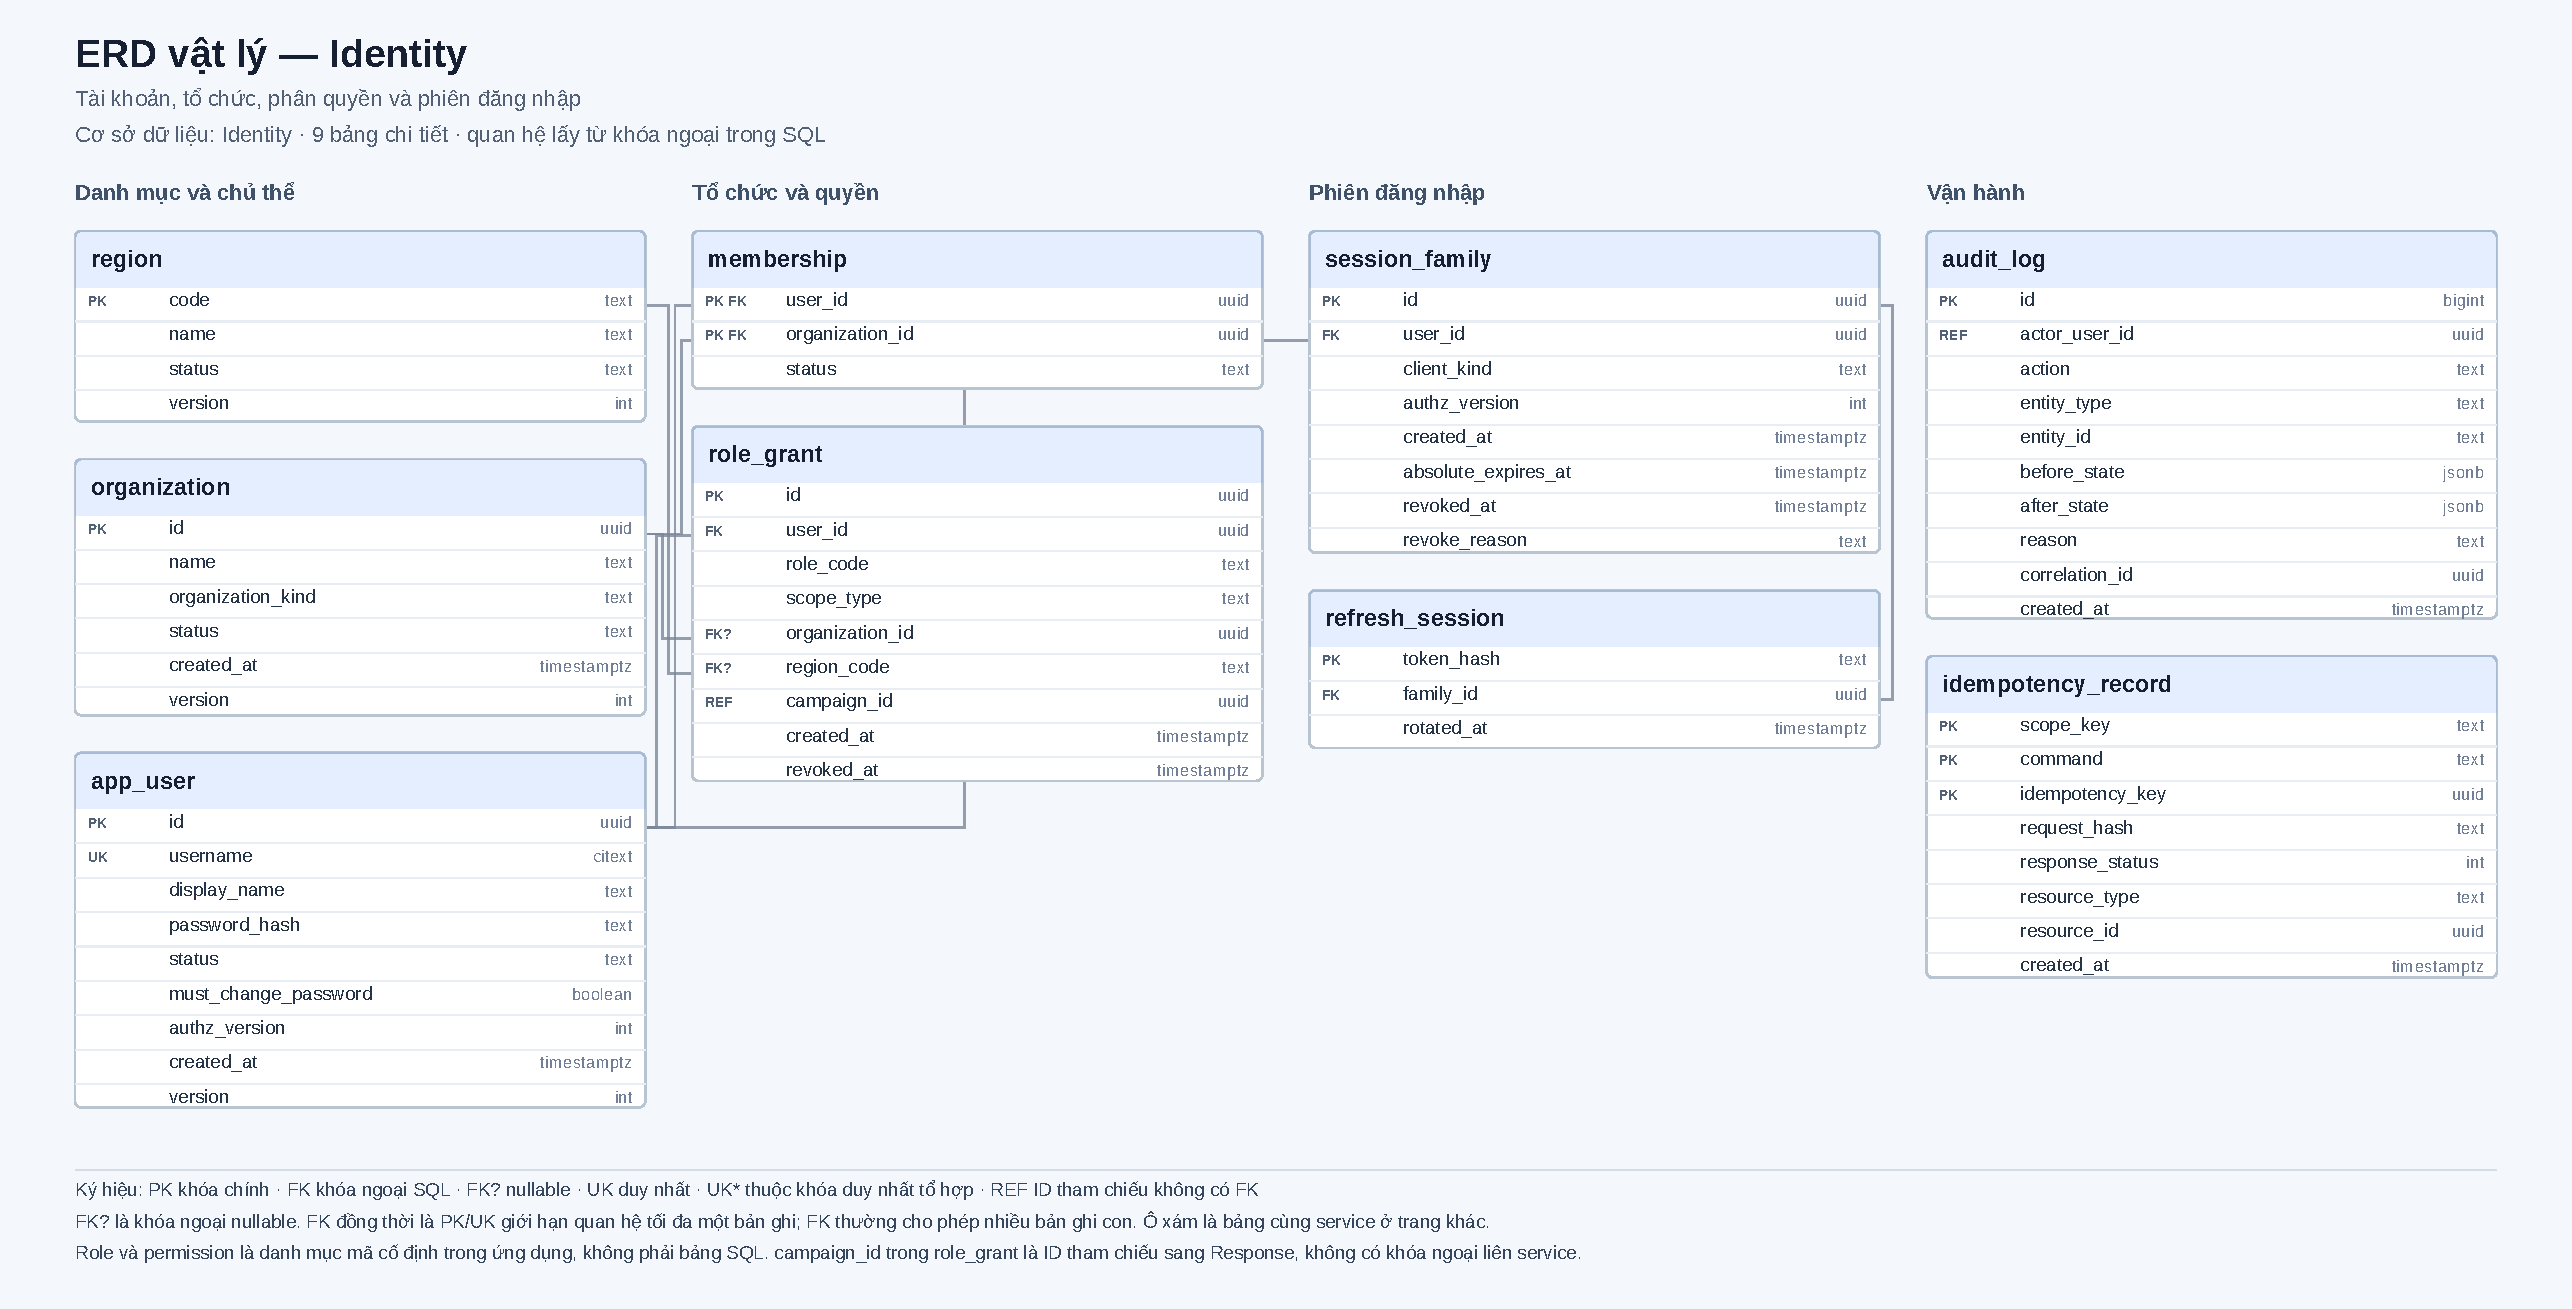
\includegraphics[width=\textwidth,height=0.78\textheight,keepaspectratio]{images/c48-erd-identity.pdf}
  \caption{ERD vật lý của cơ sở dữ liệu Identity}\label{fig:erd-identity}
  \par\small\textit{Nguồn: mô hình dữ liệu do nhóm xây dựng.}
\end{figure}
\clearpage
\begin{figure}[p]
  \centering
  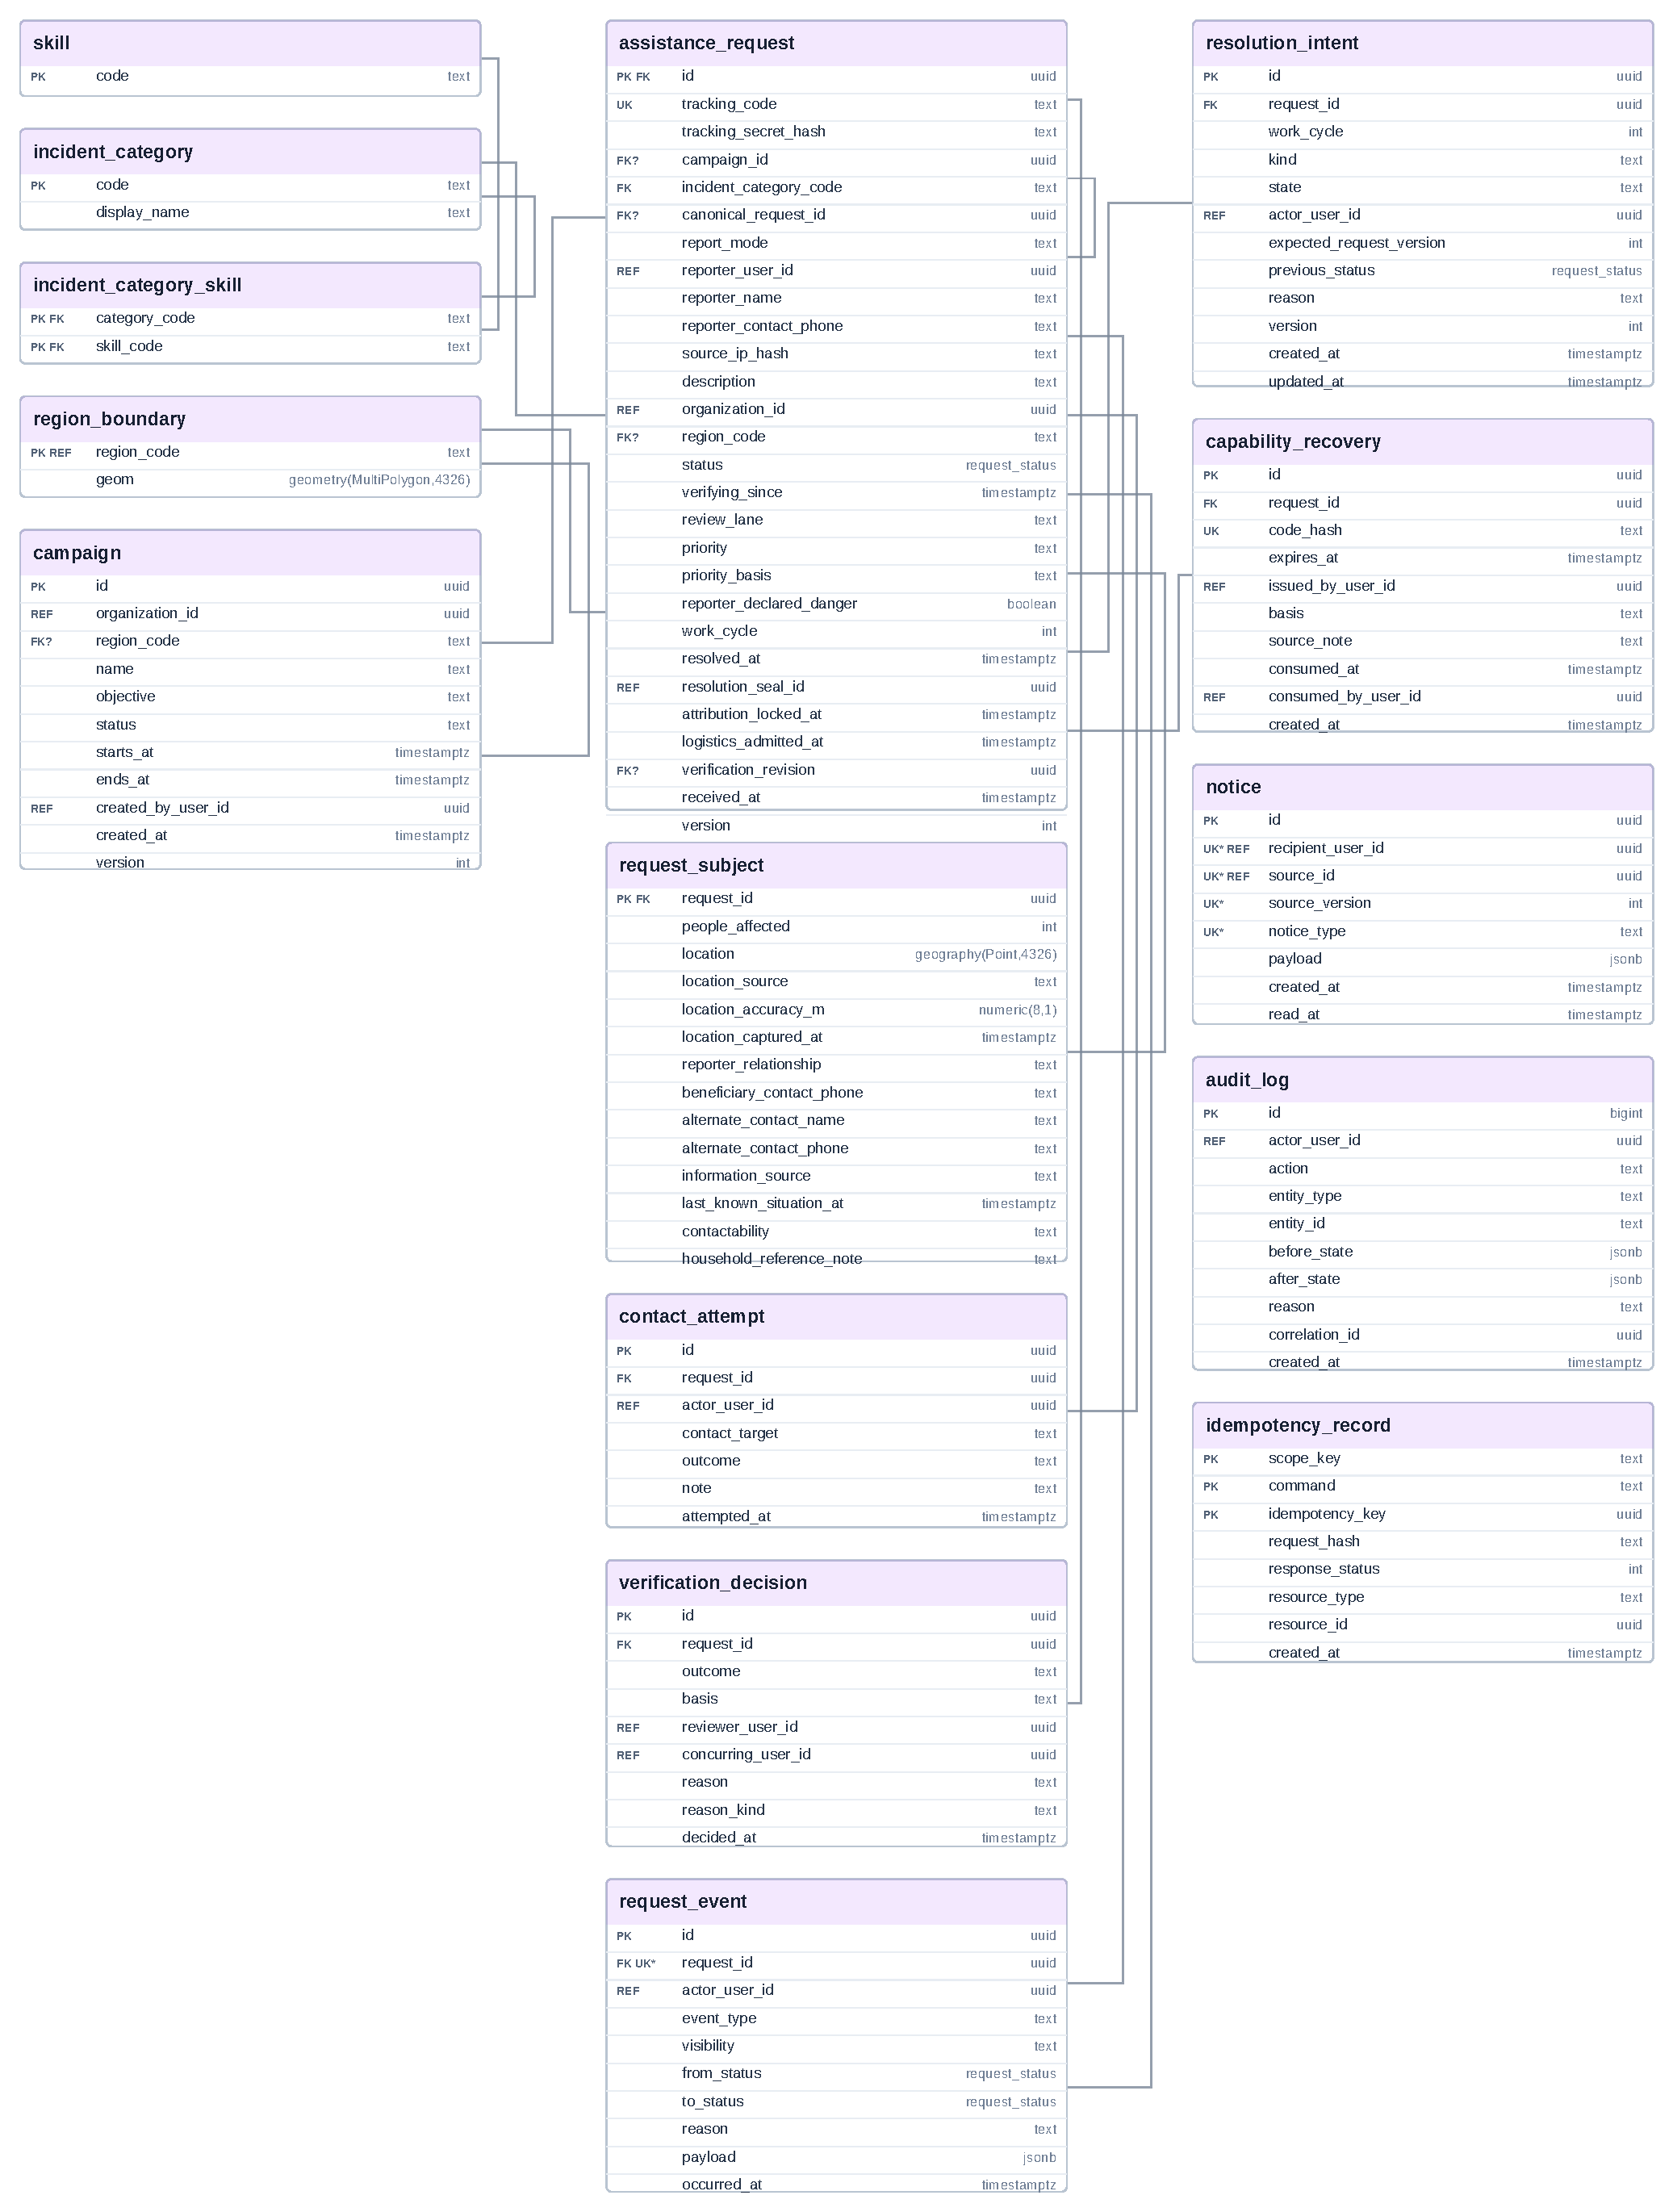
\includegraphics[width=\textwidth,height=0.78\textheight,keepaspectratio]{images/c48-erd-response-requests.pdf}
  \caption{ERD vật lý Response: tiếp nhận và theo dõi yêu cầu}\label{fig:erd-response-requests}
  \par\small\textit{Nguồn: mô hình dữ liệu do nhóm xây dựng.}
\end{figure}
\clearpage
\begin{figure}[p]
  \centering
  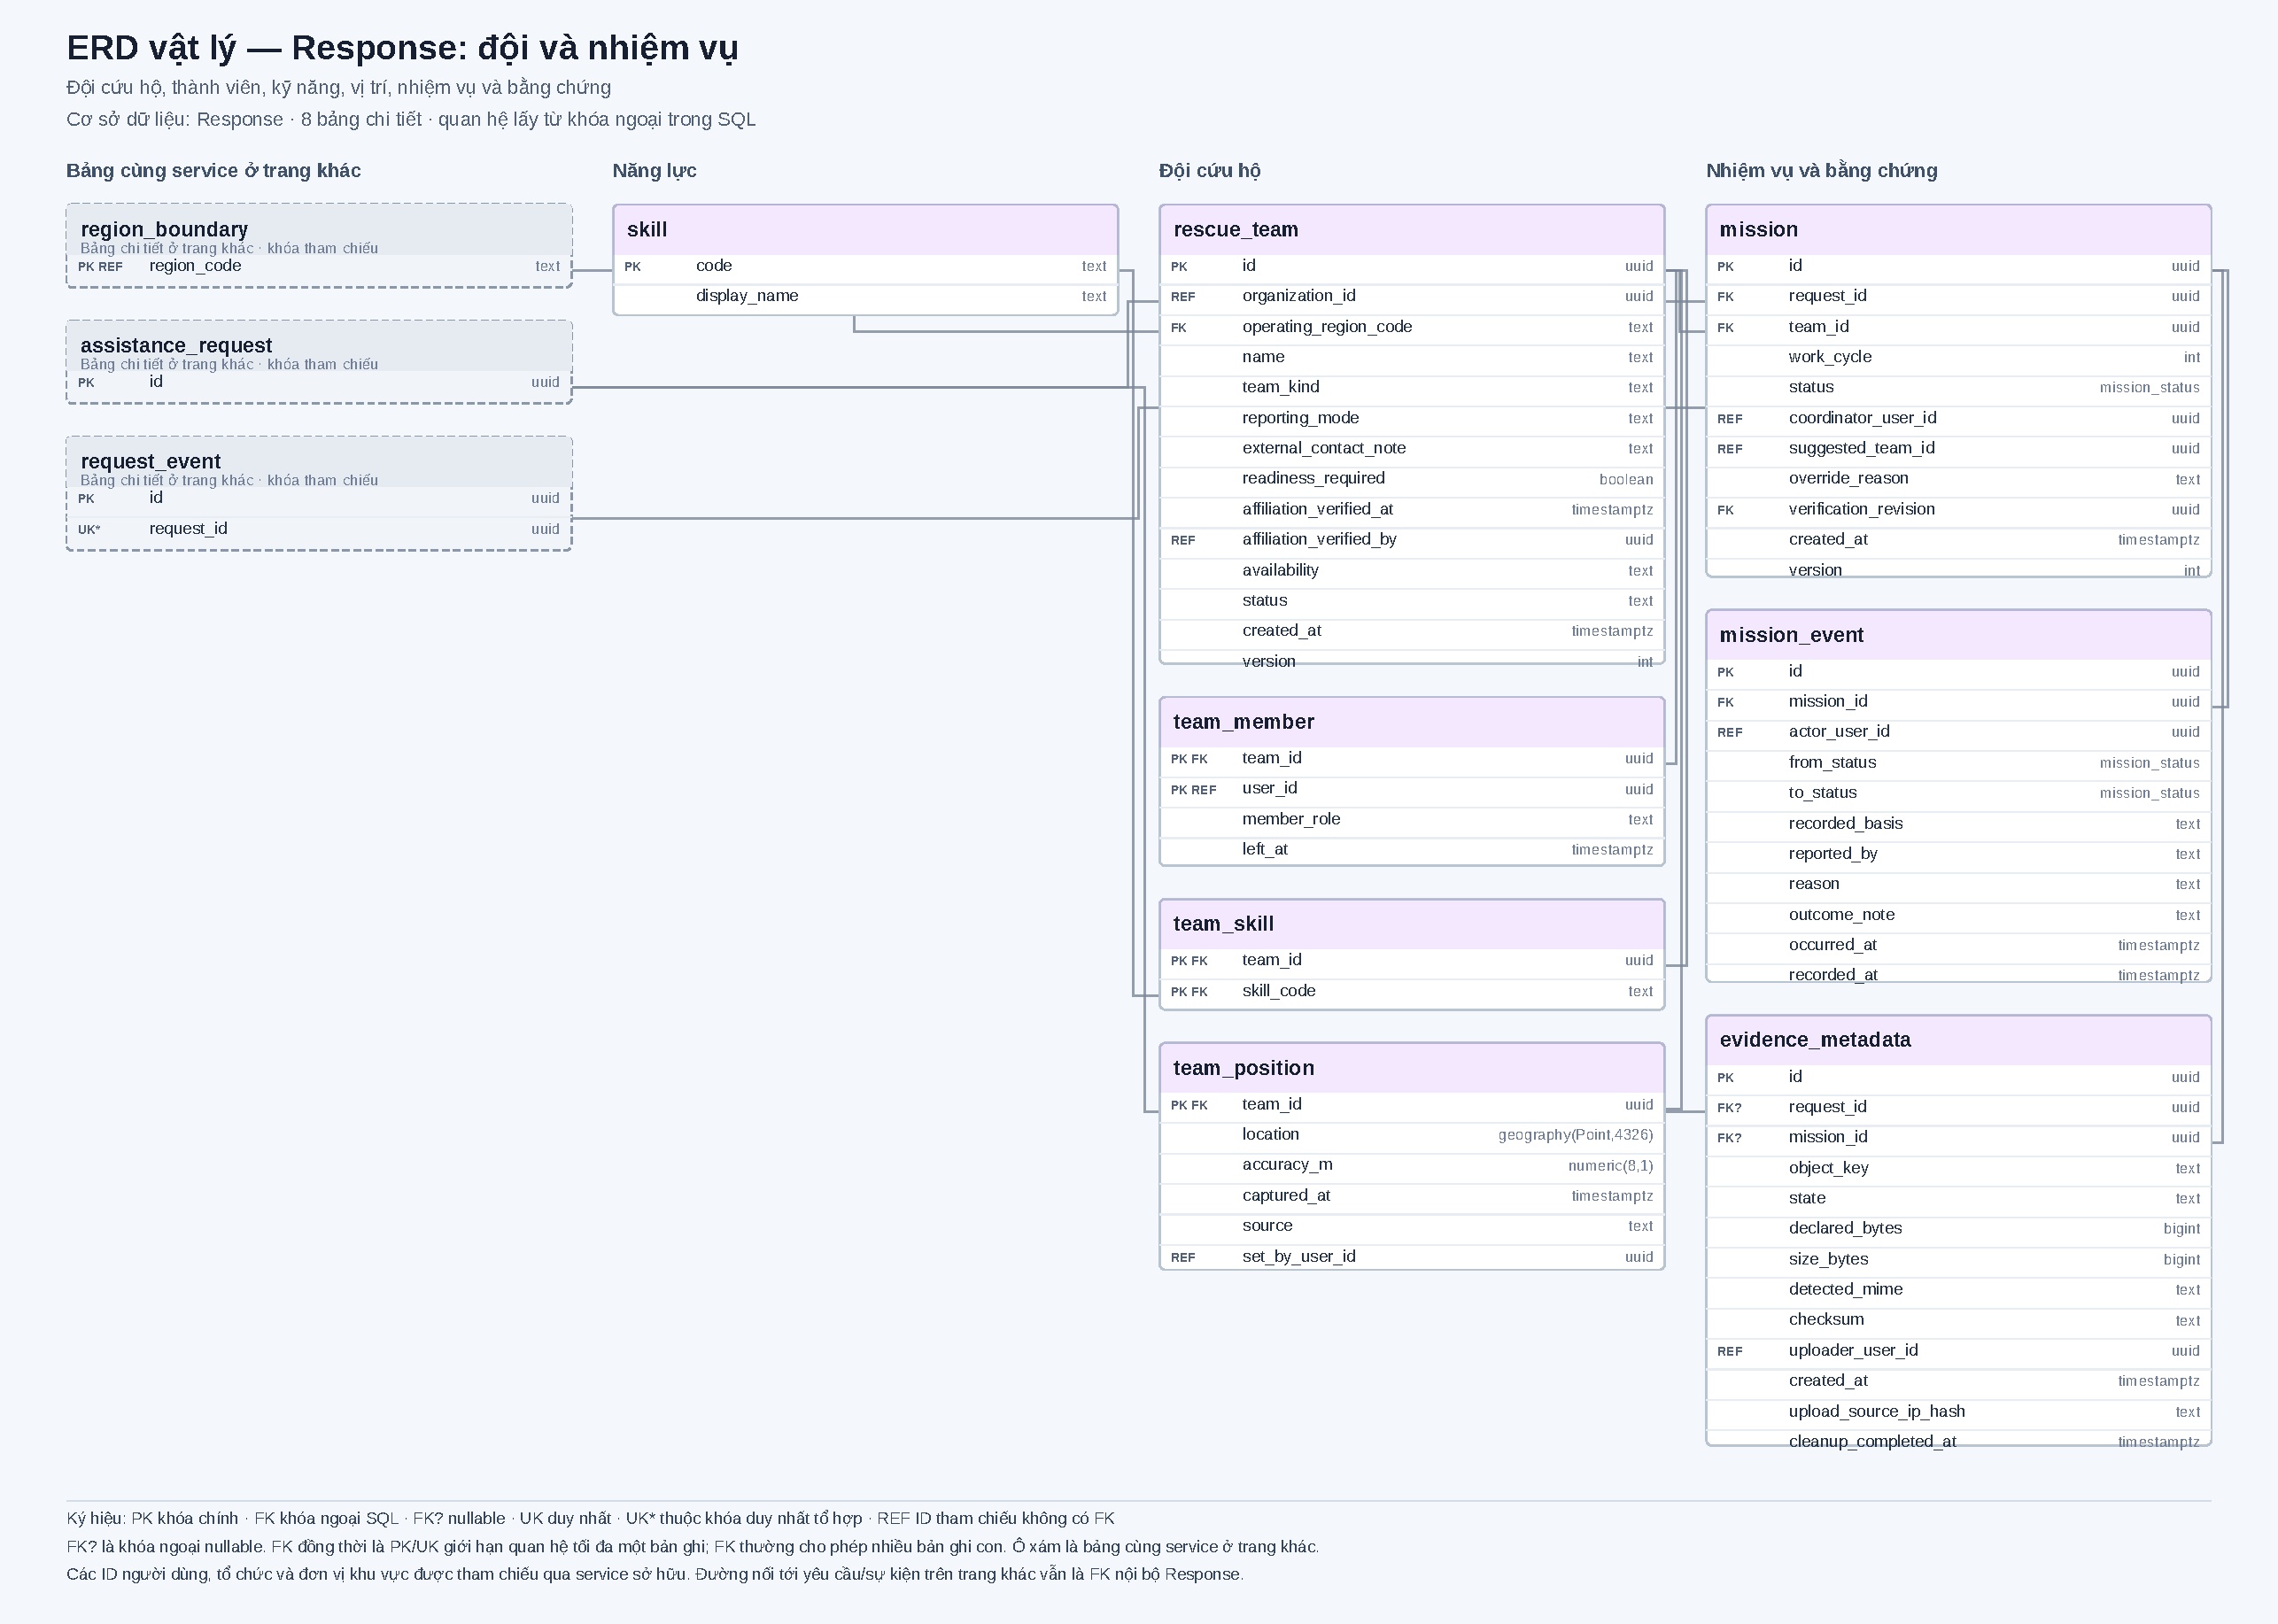
\includegraphics[width=\textwidth,height=0.78\textheight,keepaspectratio]{images/c48-erd-response-rescue.pdf}
  \caption{ERD vật lý Response: đội và hoạt động ứng cứu}\label{fig:erd-response-rescue}
  \par\small\textit{Nguồn: mô hình dữ liệu do nhóm xây dựng.}
\end{figure}
\clearpage
\begin{figure}[p]
  \centering
  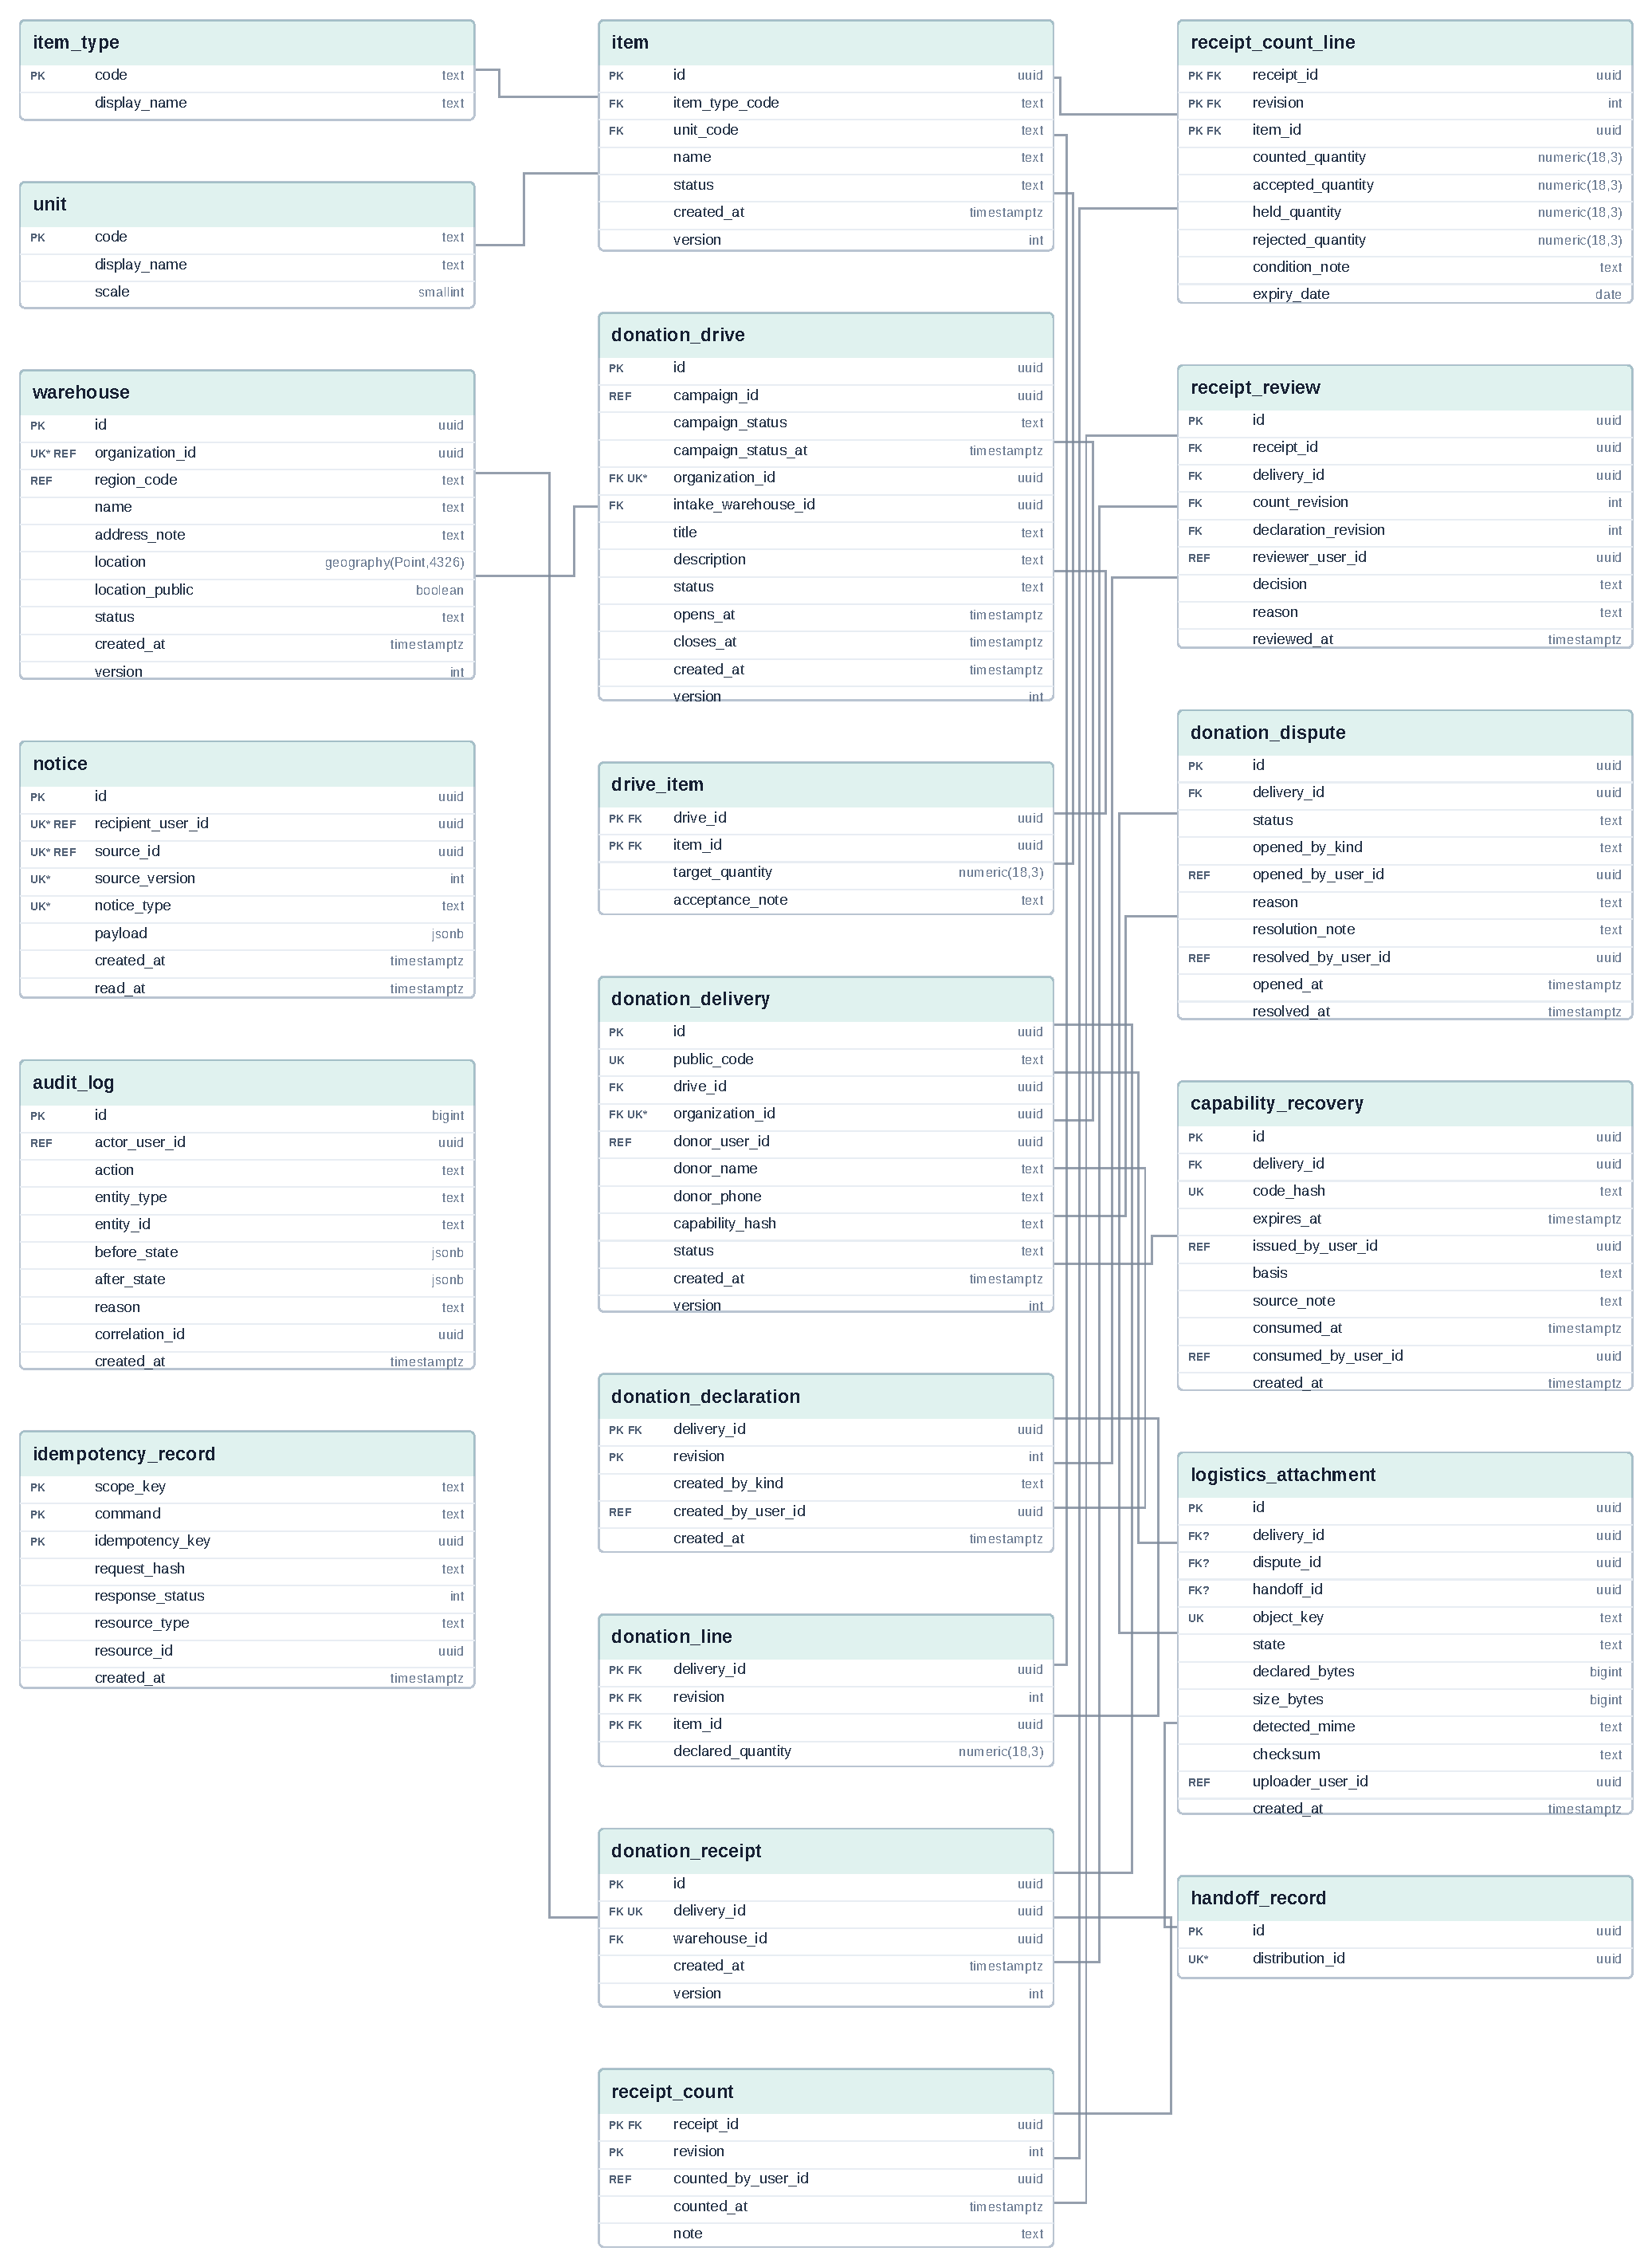
\includegraphics[width=\textwidth,height=0.78\textheight,keepaspectratio]{images/c48-erd-logistics-donations.pdf}
  \caption{ERD vật lý Logistics: đợt nhận và quyên góp hiện vật}\label{fig:erd-logistics-donations}
  \par\small\textit{Nguồn: mô hình dữ liệu do nhóm xây dựng.}
\end{figure}
\clearpage
\begin{figure}[p]
  \centering
  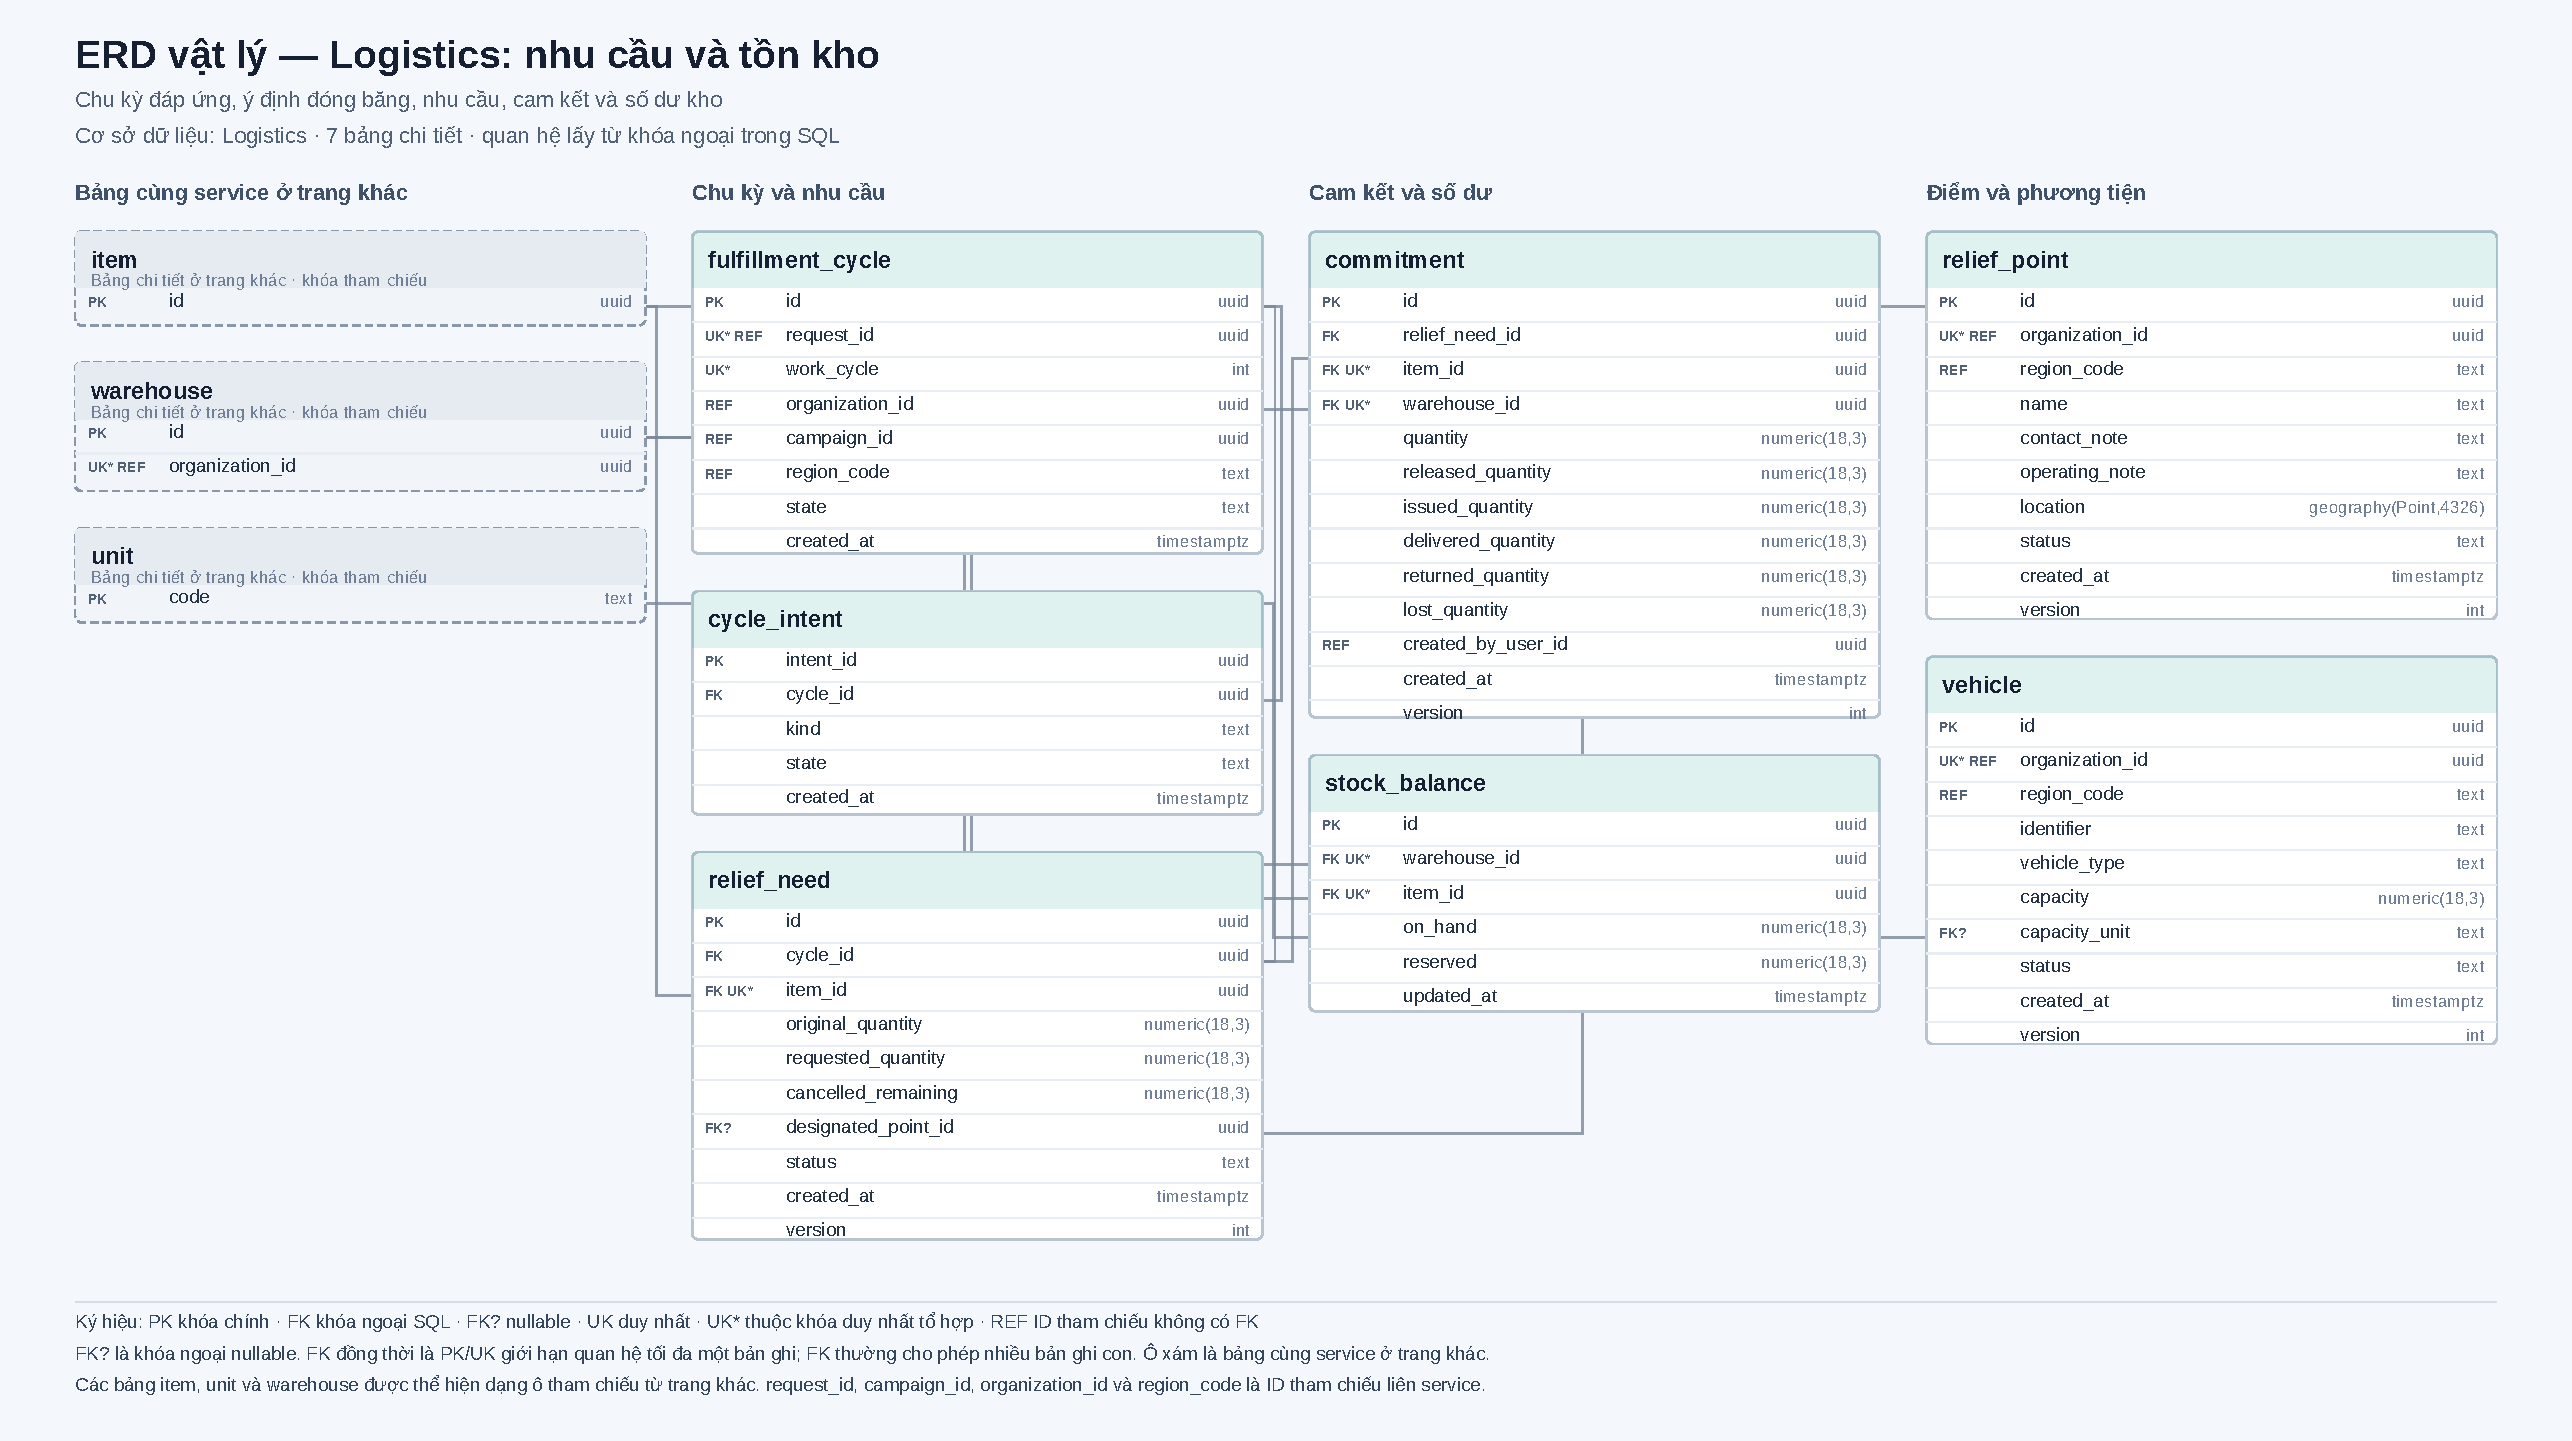
\includegraphics[width=\textwidth,height=0.78\textheight,keepaspectratio]{images/c48-erd-logistics-fulfillment.pdf}
  \caption{ERD vật lý Logistics: nhu cầu và đáp ứng cứu trợ}\label{fig:erd-logistics-fulfillment}
  \par\small\textit{Nguồn: mô hình dữ liệu do nhóm xây dựng.}
\end{figure}
\clearpage
\begin{figure}[p]
  \centering
  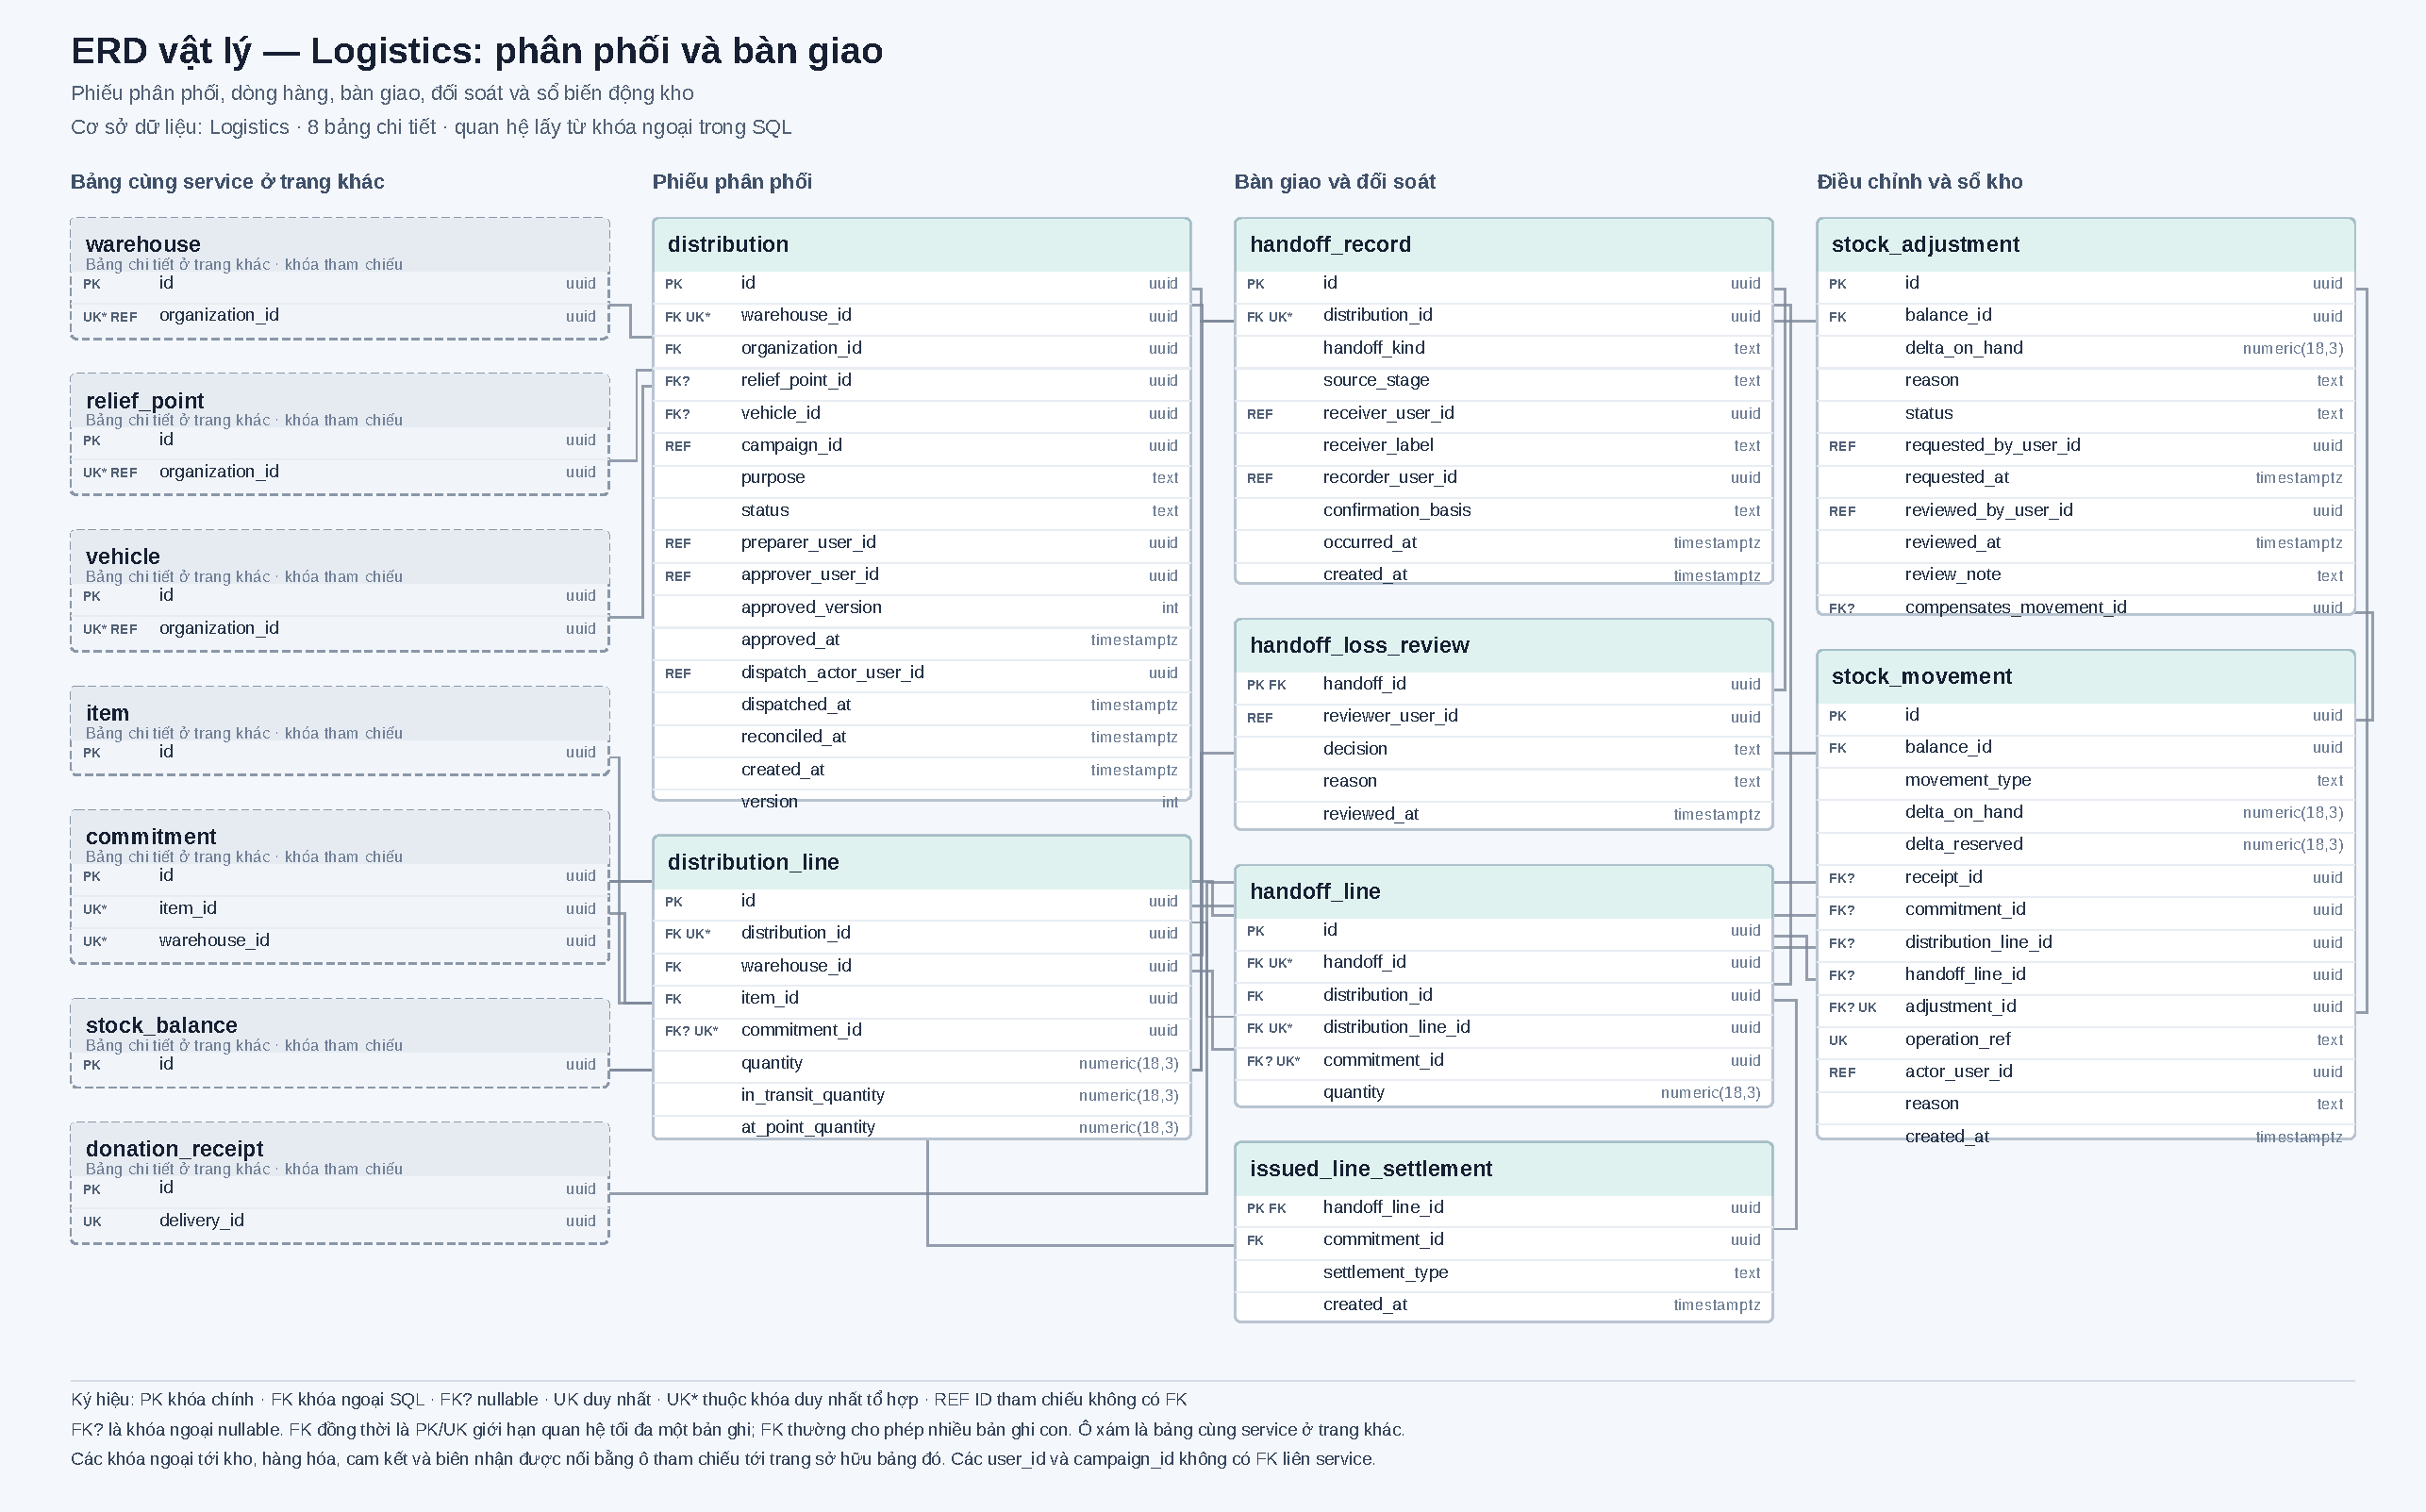
\includegraphics[width=\textwidth,height=0.78\textheight,keepaspectratio]{images/c48-erd-logistics-handoff.pdf}
  \caption{ERD vật lý Logistics: phân phối và bàn giao}\label{fig:erd-logistics-handoff}
  \par\small\textit{Nguồn: mô hình dữ liệu do nhóm xây dựng.}
\end{figure}

\chapter{THIẾT KẾ GIAO DIỆN WEB}\label{ch:web}
\section{Đăng nhập và điều hướng theo quyền}
\subsection{Giao diện đăng nhập Web}
\begin{figure}[H]
  \centering
  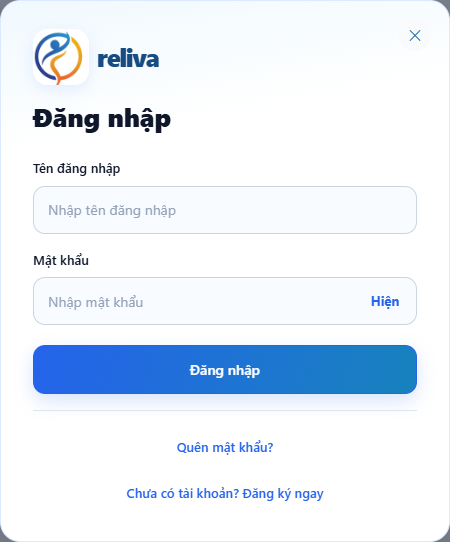
\includegraphics[width=.57\textwidth,height=.55\textheight,keepaspectratio]{images/web-login.png}
  \caption{Giao diện đăng nhập Web}\label{fig:web-login}
\end{figure}
\clearpage
\section{Giao diện người dân}
\subsection{Giao diện gửi yêu cầu SOS}
\begin{figure}[H]
  \centering
  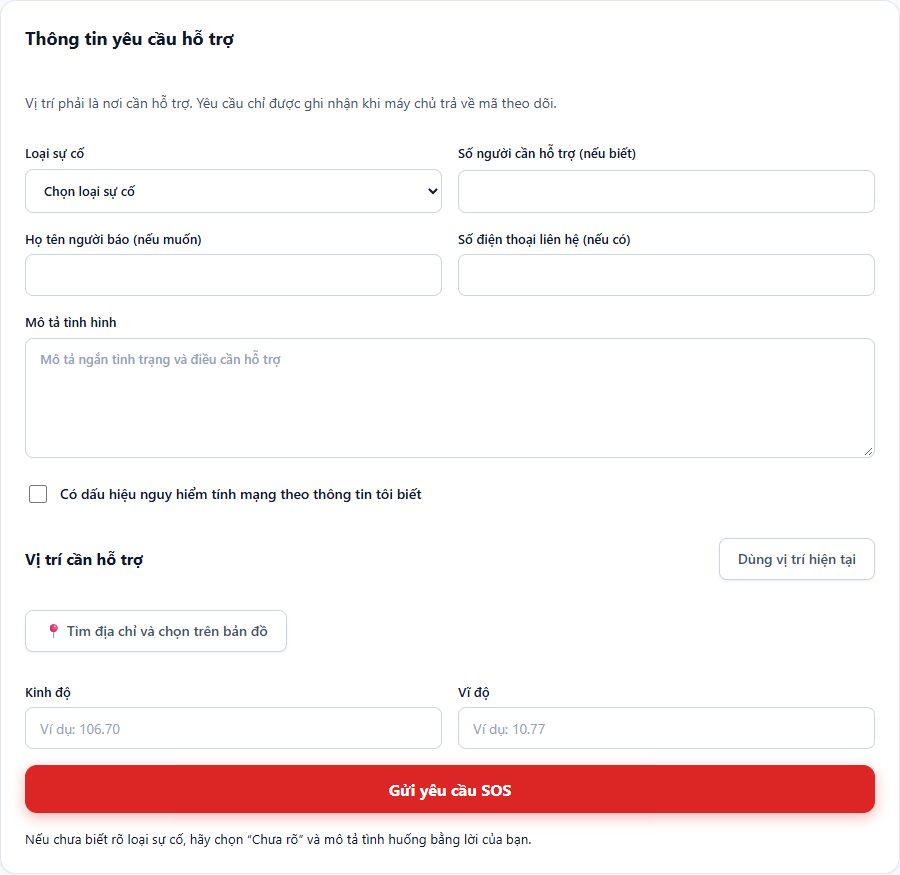
\includegraphics[width=.95\textwidth,height=.72\textheight,keepaspectratio]{images/web-citizen-sos.png}
  \caption{Giao diện gửi yêu cầu SOS trên Web}\label{fig:web-sos}
\end{figure}
\clearpage
\subsection{Giao diện đợt quyên góp hiện vật}
\begin{figure}[H]
  \centering
  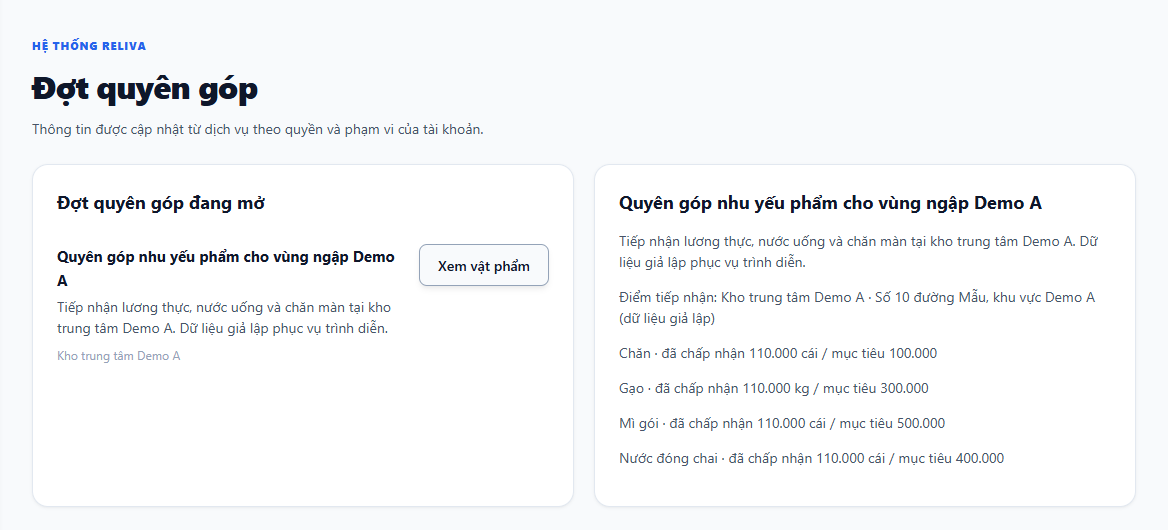
\includegraphics[width=.94\textwidth,height=.43\textheight,keepaspectratio]{images/web-donation-drive.png}
  \caption{Giao diện đợt quyên góp hiện vật trên Web}\label{fig:web-drive}
\end{figure}
\clearpage
\section{Giao diện nghiệp vụ theo vai trò}
\subsection{Giao diện hàng đợi SOS của điều phối viên}
\begin{figure}[H]
  \centering
  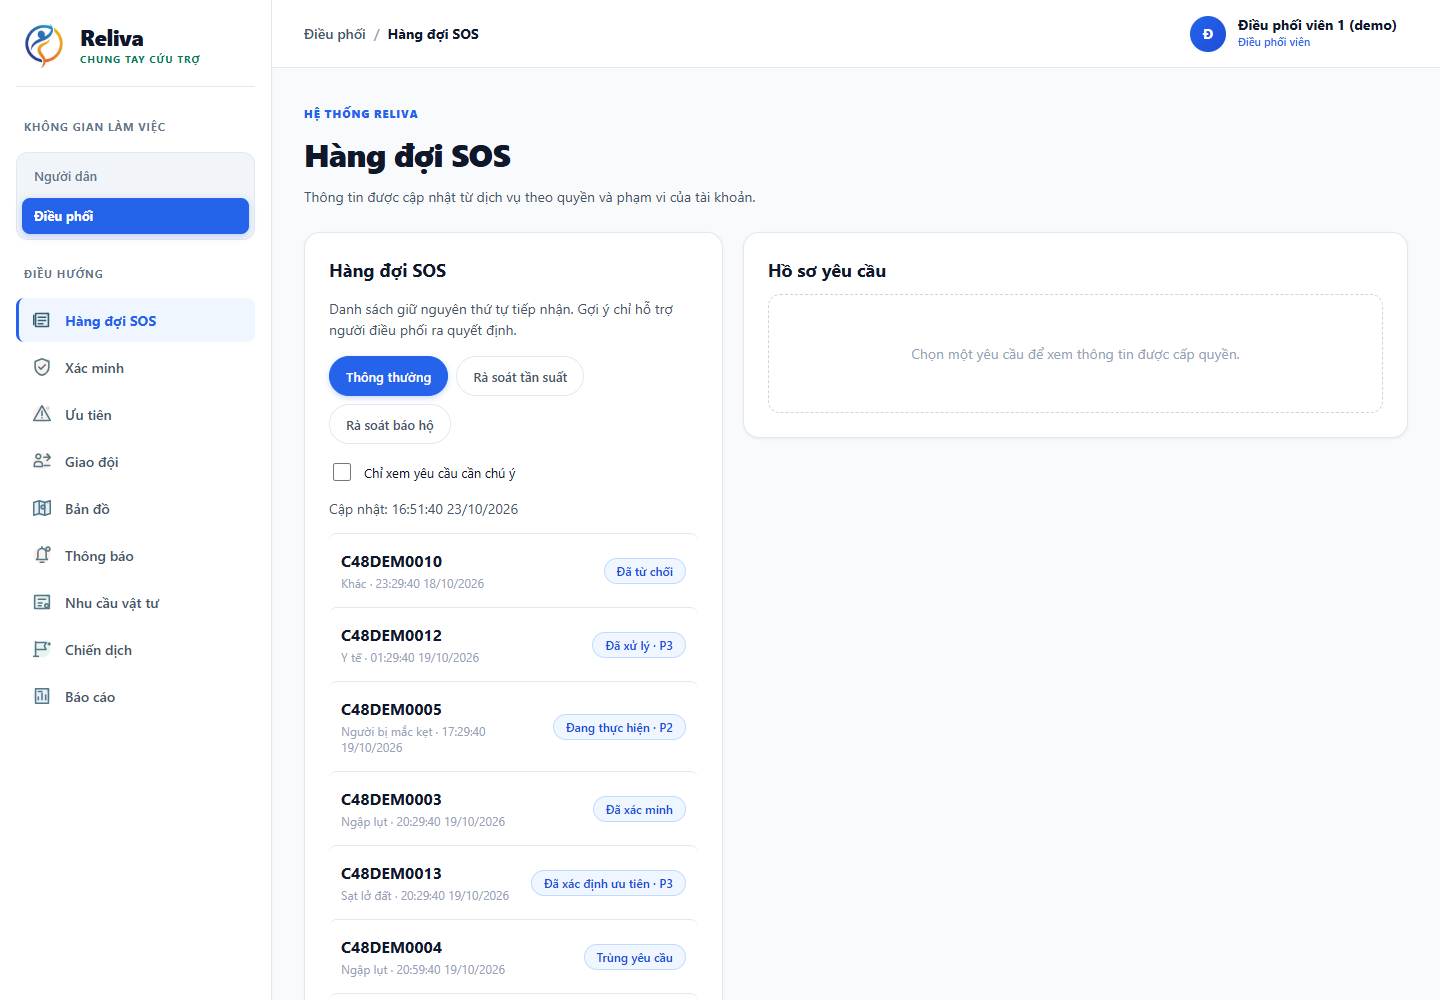
\includegraphics[width=.94\textwidth,height=.49\textheight,keepaspectratio]{images/web-coordinator-queue.png}
  \caption{Giao diện hàng đợi SOS của điều phối viên}\label{fig:web-coordinator}
\end{figure}
\clearpage
\subsection{Giao diện nhiệm vụ của đội trưởng cứu hộ}
\begin{figure}[H]
  \centering
  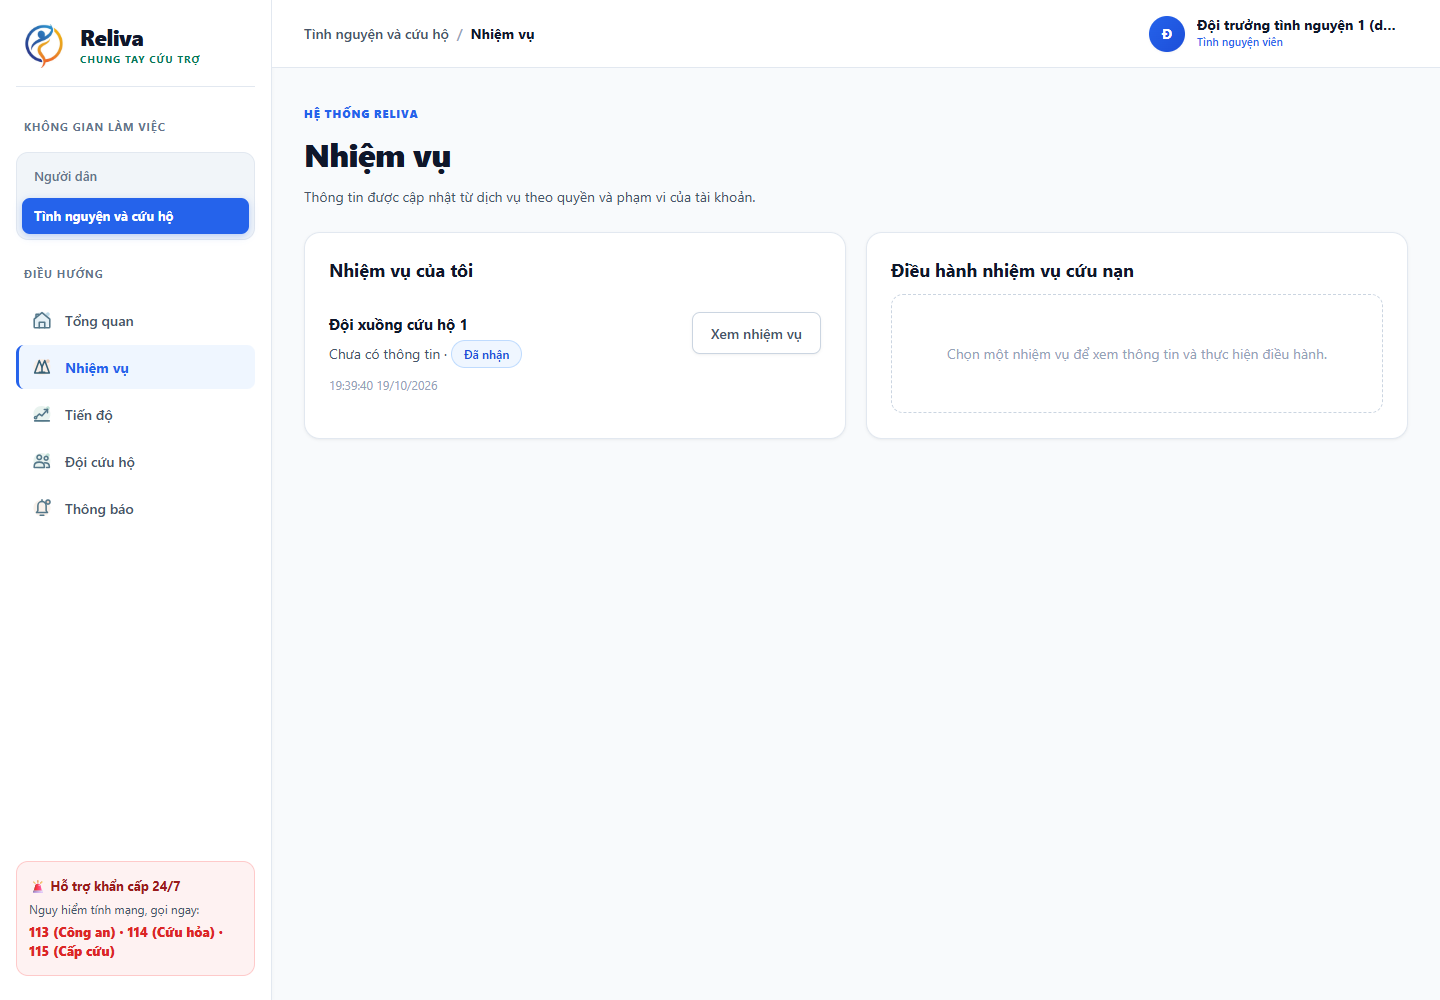
\includegraphics[width=.90\textwidth,height=.45\textheight,keepaspectratio]{images/web-volunteer-missions.png}
  \caption{Giao diện nhiệm vụ của đội trưởng cứu hộ trên Web}\label{fig:web-volunteer}
\end{figure}
\clearpage
\subsection{Giao diện bảng tồn kho cứu trợ}
\begin{figure}[H]
  \centering
  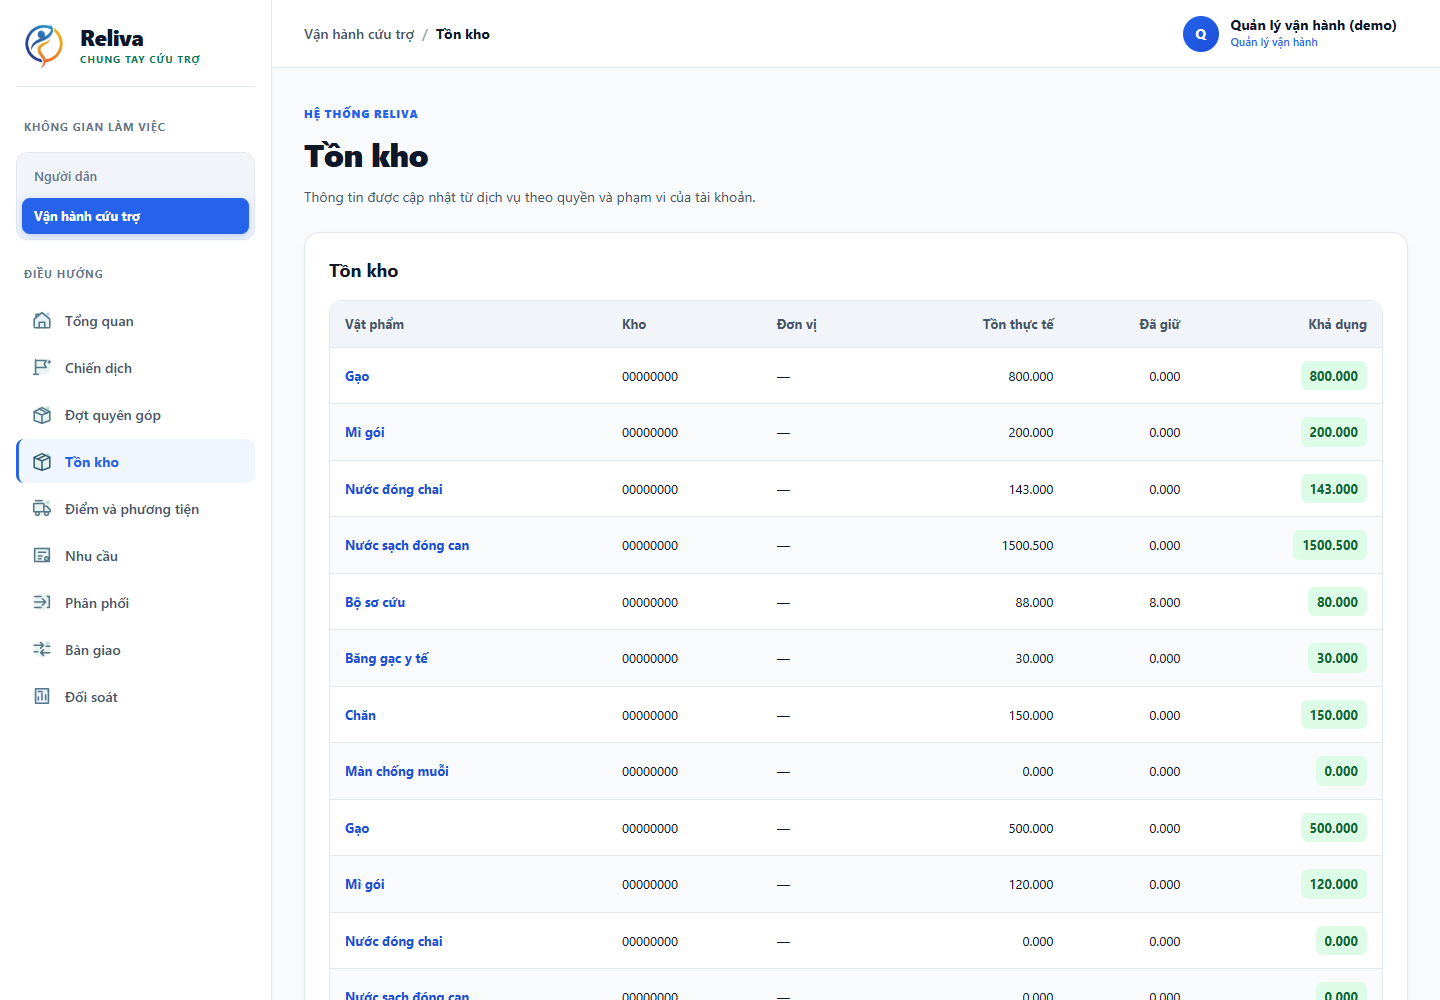
\includegraphics[width=.94\textwidth,height=.49\textheight,keepaspectratio]{images/web-operations-stock.png}
  \caption{Giao diện bảng tồn kho cứu trợ trên Web}\label{fig:web-stock}
\end{figure}
\clearpage
\subsection{Giao diện quản lý tài khoản}
\begin{figure}[H]
  \centering
  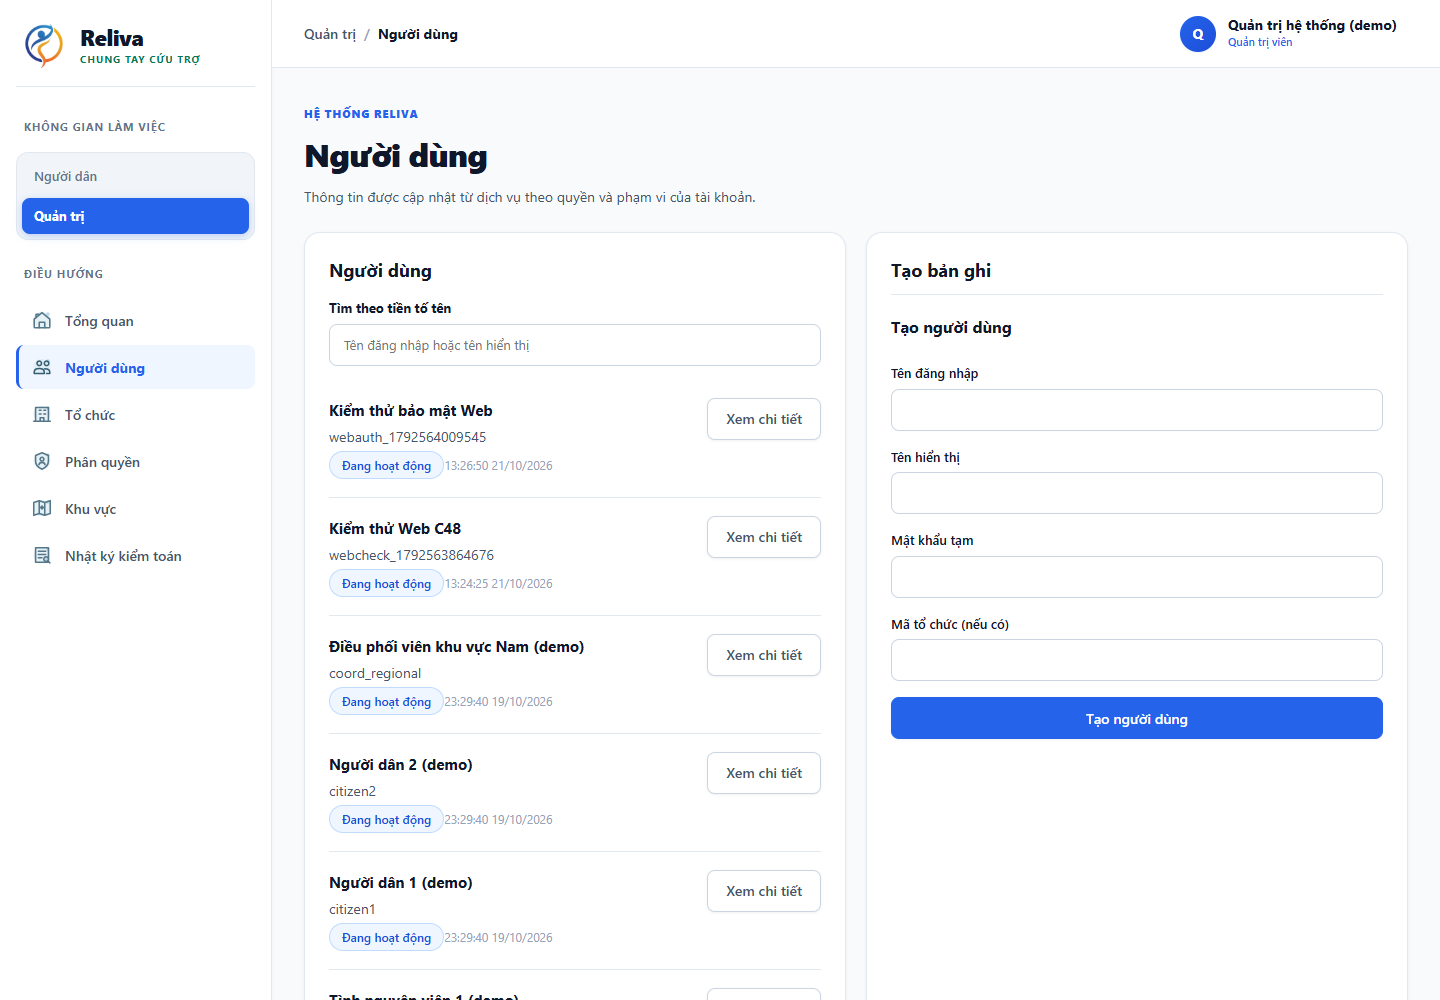
\includegraphics[width=.94\textwidth,height=.49\textheight,keepaspectratio]{images/web-admin-users.png}
  \caption{Giao diện quản lý tài khoản trên Web}\label{fig:web-admin}
\end{figure}
\clearpage

\chapter{THIẾT KẾ ỨNG DỤNG DI ĐỘNG}\label{ch:mobile}
\section{Mục tiêu và cấu trúc ứng dụng}
Ứng dụng Mobile được xây dựng bằng React Native, Expo và TypeScript, kết nối các API Identity, Response và Logistics. Hai nhóm thao tác chính là báo cứu trợ của người dân (UR-01, UR-02) và xử lý nhiệm vụ của đội cứu hộ (UR-04); quyên góp hiện vật đáp ứng UR-08 ở phía người tặng. Giao diện hiển thị trạng thái bằng tiếng Việt; mã trạng thái, mã lỗi và tên trường API vẫn là định danh kỹ thuật để ứng dụng xử lý ổn định. Các màn hình dưới đây minh họa sản phẩm với dữ liệu demo; ảnh chụp không tự chứng minh toàn bộ luồng đã được kiểm thử đầu cuối.

\begin{table}[htbp]
  \centering
  \caption{Đối chiếu màn hình Mobile với nghiệp vụ và dịch vụ}\label{tab:mobile-screens}
  \small
  \begin{tabularx}{\textwidth}{@{}L{3cm}Y L{2cm}@{}}
    \toprule
    \textbf{Nhóm màn hình} & \textbf{Thông tin và thao tác chính} & \textbf{Dịch vụ} \\
    \midrule
    Đăng nhập, đổi mật khẩu & Xác thực tài khoản, cập nhật mật khẩu khi có yêu cầu. & Identity \\
    Trang chủ, SOS, bản đồ & Chọn SELF hoặc PROXY, ghi nhận tình huống và vị trí hiện trường. & Response \\
    Theo dõi, bổ sung & Xem mã tra cứu, tiến trình và gửi thông tin mới. & Response \\
    Quyên góp & Xem đợt nhận, khai báo hiện vật và theo dõi kiểm đếm. & Logistics \\
    Bảng đội và nhiệm vụ & Xem trạng thái đội, danh sách và chi tiết nhiệm vụ. & Response \\
    \bottomrule
  \end{tabularx}
  \par\small\textit{Nguồn:} Nhóm thực hiện đối chiếu ảnh chụp và mã nguồn Mobile.
\end{table}

\section{Xác thực và điều hướng theo vai trò}
\subsection{Giao diện đăng nhập}
\mobilescreenshot{images/đăng nhập.jpg}{Giao diện đăng nhập Mobile, đã cắt phần thông tin tài khoản thử nghiệm}{fig:mobile-login}
\clearpage
\subsection{Giao diện đổi mật khẩu}
\mobilescreenshot{images/Đổi mật khẩu.jpg}{Giao diện đổi mật khẩu trên Mobile}{fig:mobile-password}
\clearpage
\section{Luồng SOS của người dân}
\subsection{Giao diện trang chủ và lựa chọn cách báo}
\mobilescreenshot{images/trang chủ.jpg}{Giao diện trang chủ và lựa chọn cách gửi tin báo}{fig:mobile-home}
\clearpage
\subsection{Giao diện báo cứu nạn tại chỗ}
\mobilescreenshot{images/thông tin liên hệ.jpg}{Giao diện báo cứu nạn tại chỗ}{fig:mobile-sos}
\clearpage
\subsection{Giao diện ghim vị trí cứu nạn trên bản đồ}
\mobilescreenshot{images/map.jpg}{Giao diện ghim vị trí cứu nạn trên bản đồ}{fig:mobile-map}
\clearpage
\subsection{Giao diện tra cứu tiến độ cứu hộ}
\mobilescreenshot{images/mã cứu trợ.jpg}{Giao diện tra cứu tiến độ cứu hộ}{fig:mobile-status}
\clearpage
\subsection{Giao diện bổ sung tình hình và ảnh hiện trường}
\mobilescreenshot{images/bằng chứng.jpg}{Giao diện bổ sung tình hình và ảnh hiện trường}{fig:mobile-evidence}
\clearpage
\section{Quyên góp hiện vật trên Mobile}
\subsection{Giao diện quyên góp cứu trợ}
\mobilescreenshot{images/quyên góp cứu trợ.jpg}{Giao diện quyên góp cứu trợ}{fig:mobile-donations}
\clearpage
\subsection{Giao diện khai báo bàn giao hiện vật}
\mobilescreenshot{images/Khai báo bàn giao.jpg}{Giao diện khai báo bàn giao hiện vật}{fig:mobile-handover}
\clearpage
\section{Không gian đội trưởng và nhiệm vụ cứu hộ}
\subsection{Giao diện bảng điều khiển đội trưởng}
\mobilescreenshot{images/Bảng điều khiển đội trưởng.jpg}{Giao diện bảng điều khiển đội trưởng}{fig:mobile-leader}
\clearpage
\subsection{Giao diện danh sách nhiệm vụ}
\mobilescreenshot{images/Danh sách nhiệm vụ.jpg}{Giao diện danh sách nhiệm vụ cứu hộ}{fig:mobile-missions}
\clearpage
\subsection{Giao diện chi tiết nhiệm vụ}
\mobilescreenshot{images/Chi tiết nhiệm vụ.jpg}{Giao diện chi tiết nhiệm vụ cứu hộ}{fig:mobile-mission-detail}
\clearpage
\chapter{KẾT LUẬN VÀ KIẾN NGHỊ}\label{ch:conclusion}
\section{Kết quả đạt được}
Nhóm đã phân tích nhu cầu của các tác nhân, xác định yêu cầu, xây dựng kiến trúc ba dịch vụ và mô hình dữ liệu cho các nghiệp vụ chính. Backend hiện thực các chức năng quản lý tài khoản và quyền, tiếp nhận và điều phối yêu cầu SOS, theo dõi nhiệm vụ ứng cứu, quản lý chiến dịch, tiếp nhận hàng cứu trợ, kiểm đếm, tồn kho và phân phối. Web đã tích hợp các luồng chính theo vai trò, với kiểm tra trình duyệt giới hạn cho một số luồng công khai và tài khoản. Mobile đã xây dựng các màn hình báo cứu trợ, theo dõi, quyên góp và nhiệm vụ đội; bộ ảnh demo minh họa giao diện của các luồng đó. Các thao tác quan trọng được lưu lại để hỗ trợ kiểm tra và đối soát.

\section{Giới hạn còn lại}
Hệ thống hiện được xây dựng và minh họa trong môi trường demo, chưa được kiểm chứng qua một đợt ứng phó thiên tai thực tế. Kiểm thử tự động và một số luồng tích hợp đã được thực hiện, nhưng bằng chứng đầu cuối cho toàn bộ thao tác ghi của từng vai trò vẫn chưa đầy đủ. Các tình huống mất mạng, gửi lại yêu cầu, quyền GPS và máy ảnh, cũng như khả năng tiếp cận trên nhiều thiết bị cần được kiểm tra thêm; đồng bộ ngoại tuyến nâng cao và thông báo đẩy chưa hoàn thiện.

Ở tầng vận hành, nhóm chưa hoàn tất kiểm chứng quyền truy cập tệp riêng tư, sao lưu và khôi phục dữ liệu, tác vụ định kỳ và hiệu năng trên dữ liệu đại diện. Các ngưỡng ưu tiên, phạm vi chia sẻ vị trí, thời hạn lưu dữ liệu và quy trình phối hợp với lực lượng ngoài hệ thống vẫn cần được người có thẩm quyền xác nhận trước khi áp dụng thực tế. Bộ tài liệu SRS, SDD, ca kiểm thử, hướng dẫn cài đặt và hướng dẫn người dùng cũng cần được hoàn thiện để bàn giao đầy đủ.

\section{Kiến nghị}
\begin{enumerate}
  \item Kiểm chứng các thao tác ghi Web và Mobile còn lại với API thật; bổ sung biên bản cho tình huống bình thường, lỗi và mất kết nối.
  \item Kiểm tra quyền truy cập tệp, sao lưu và khôi phục, tác vụ định kỳ, cũng như hiệu năng của API và báo cáo trên dữ liệu đại diện.
  \item Hoàn thiện SRS, SDD, bộ ca kiểm thử, hướng dẫn cài đặt và hướng dẫn người dùng; duy trì mã UR/FR/NFR/UC/TC để đối chiếu yêu cầu với kết quả.
  \item Trao đổi với giảng viên hướng dẫn và đơn vị nghiệp vụ để xác nhận các quy tắc ưu tiên, quyền xem vị trí và thời hạn lưu dữ liệu trước khi dùng với tình huống thực tế.
\end{enumerate}

\begin{thebibliography}{99}
  \addcontentsline{toc}{chapter}{\bibname}
  \bibitem{ocha-hpc} United Nations Office for the Coordination of Humanitarian Affairs (OCHA), \textit{About the Humanitarian Programme Cycle}, \url{https://knowledge.base.unocha.org/wiki/spaces/hpc/pages/3993075713}, truy cập ngày 23/10/2026.
  \bibitem{ocha-data} OCHA Centre for Humanitarian Data, \textit{OCHA Data Responsibility Guidelines 2025}, \url{https://centre.humdata.org/data-responsibility-guidelines-2025/}, truy cập ngày 23/10/2026.
  \bibitem{wfp-warehouse} Logistics Cluster, \textit{Warehousing Documentation}, \url{https://log.logcluster.org/en/warehousing-documentation}, truy cập ngày 23/10/2026.
  \bibitem{owasp-bola} OWASP, \textit{API1:2023 Broken Object Level Authorization}, \url{https://api-security.owasp.org/editions/2023/en/0xa1-broken-object-level-authorization/}, truy cập ngày 23/10/2026.
  \bibitem{nestjs} NestJS, \textit{First steps}, \url{https://docs.nestjs.com/first-steps}, truy cập ngày 23/10/2026.
  \bibitem{typeorm} TypeORM, \textit{Postgres / CockroachDB}, \url{https://typeorm.io/docs/drivers/postgres/}, truy cập ngày 23/10/2026.
  \bibitem{postgis} PostGIS Project, \textit{PostGIS Manual}, \url{https://postgis.net/docs/}, truy cập ngày 23/10/2026.
  \bibitem{react} React, \textit{Describing the UI}, \url{https://react.dev/learn/describing-the-ui}, truy cập ngày 23/10/2026.
  \bibitem{vite} Vite, \textit{Getting Started}, \url{https://vite.dev/guide/}, truy cập ngày 23/10/2026.
  \bibitem{expo-location} Expo, \textit{Location}, \url{https://docs.expo.dev/versions/latest/sdk/location/}, truy cập ngày 23/10/2026.
  \bibitem{docker-compose} Docker, \textit{Docker Compose}, \url{https://docs.docker.com/compose/}, truy cập ngày 23/10/2026.
  \bibitem{minio} MinIO, \textit{AIStor Subscriptions \& Pricing}, \url{https://www.min.io/pricing}, truy cập ngày 23/10/2026.
\end{thebibliography}

\end{document}
